% \pagebreak[4]
% \hspace*{1cm}
% \pagebreak[4]
% \hspace*{1cm}
% \pagebreak[4]


\newenvironment{minipeqn}[1][]{\begin{minipage}[#1]{.75\textwidth}\begin{equation}}{\end{equation}\end{minipage}}

\ifpdf
    \graphicspath{{Chapter1/Chapter1Figs/PNG/}{Chapter1/Chapter1Figs/PDF/}{Chapter1/Chapter1Figs/}}
\else
    \graphicspath{{Chapter1/Chapter1Figs/EPS/}{Chapter1/Chapter1Figs/}}
\fi

\chapter{The special linear group $\sltz$}

\section{Introduction}


\begin{definition}
The special linear group of degree two over the ring of integers is 
$$\sltz = \left\lbrace \abcd \, \vert \, a,b,c,d \in \mathbb{Z}\, ad-bc =1 \right\rbrace$$
\end{definition}
The set $\sltz$ forms a group under matrix multiplication since, matrix multiplication is associative, $I_2 = \left(\begin{array}{ c c }  1 & 0 \\ 0 & 1 \end{array} \right) \in \sltz$, the inverse of $\abcd = \left(\begin{array}{ c c }  d & -b \\ -c & a \end{array} \right)$, it is closed under multiplication since $\det(AB) = \det(A)\det(B) = 1$ for $A,B \in \sltz$.\\
\\


The two most important matrices for $\sltz$ are $S = \sm$ and $T = \tm$. The matrix $S$ has order $4$ and $S^2 = -I_2$. For $T$ we have $T^n = \left(\begin{array}{ c c } 1 & n \\ 0 & 1 \end{array} \right)$ for $n \in \mathbb{Z}$, so the matrix $T$ has infinite order.
In words, left multiplication by $S$ swaps the rows of a matrix and changes the sign of the new top row. Left multiplication by $T$ adds the bottom row to the top row and leaves the bottom row unchanged.
$$S\abcd = \left(\begin{array}{ c c }  -c & -d \\ a & b \end{array} \right)\,,\quad 
T^n\abcd = \left(\begin{array}{ c c }  a +cn & b+dn \\ c & d \end{array} \right).$$

\begin{theorem}\label{thm:STGenerateSLTZ}
The group $\sltz$ is generated by $S$ and $T$. 
\end{theorem}
This theorem is central to the study of $\sltz$, most of the results in this report make use of it. There are two common methods to prove this, one geometric and the other algebraic given in subsection \ref{subsect:proofAlgebraicSTGenerate}.

\section{Möbius transformations}

In this section we discuss a geometric approach to $\sltz$, we give a version of the classic geometric proof of Theorem \ref{thm:STGenerateSLTZ}. Some of the exposition on Möbius transformations was derived from University of Manchester hyperbolic geometry course notes \citep{manchesterNotes}
\\

\begin{definition}
The upper half-plane is the set of complex numbers with positive imaginary part:
$$ \mathcal{H} : = \{ z  = x + iy \in \mathbb{C} \, : \, y > 0\}$$ 
\end{definition}

\begin{definition}

Let $a,b,c,d \in \mathbb{R}$ such that $ad -bc >0 \in \mathbb{R}$, and define the map

\begin{align*}
\gamma \, : \, \mathcal{H} \rightarrow \mathcal{H} \\
\gamma(z) = \frac{az + b}{cz +d}
\end{align*}

The map $\gamma$ is called a Möbius transformation of $\mathcal{H}$. The set of these Möbius transformations is denoted $\mobh$
\end{definition}

\begin{remark}\label{rem:mobiusExpandBiject}
Let $ \gamma = \frac{az + b}{cz +d} \in \mobh$ and let $z \in \mathcal{H}$. 
Expanding out $\gamma(z)$ we get, 

\begin{equation}\label{eqn:mobexpanded}
\begin{split}
\gamma z &=  \frac{az +b}{cz+d}   =  \frac{ax + aiy + b}{cx + ciy + d}  =  \frac{(ax+aiy + b)(cx +d - ciy}{{(cx+d)}^2 + {(cy)}^2} \\ 
						& = \frac{ac(x^2 + y^2) + x(ad+bc) + bd}{{|cz+d|}^2} + i\frac{y(ad-bc)}{{|cz+d|}^2}
\end{split}
\end{equation}
Focusing on the imaginary part in equation \ref{eqn:mobexpanded} we see that the image of a Möbius transformation of $\mathcal{H}$ does indeed lie in $\mathcal{H}$,
\begin{equation}\label{eqn:imaginaryMobius}
Im(\gamma z) = \frac{Im(z)(ad-bc)}{{|cz+d|}^2} > 0
\end{equation}
We can actually go further to say that $\gamma \in \mobh$ is a bijective map from $\mathcal{H}$ to itself, we can show this by finding the inverse of $\gamma$ in $\mobh$.  Let $g= \frac{dz - b }{-cz + a}$, first we note $da - (-b)(-c) = ad - bc > 0$ so $g \in \mobh$. We can show $g$ is a left inverse directly,
\begin{align*}
\gamma^{-1}\gamma(z) &= \gamma^{-1}(\frac{az +b}{cz+d}) = \frac{d\frac{az +b}{cz+d} -b}{-c \frac{az +b}{cz+d} + a} \\
& = \frac{ \frac{d(az +b) - b(cz + d)}{cz + d}}{\frac{-c(az +b) + a(cz +d)}{cz+d}} = \frac{ daz +db - bcz -bd}{-caz -cb + acz +ad} \\
& = \frac{(da - bc)z}{-cb  +ad} \\
& = z
\end{align*}
By a similar computation we can show $g$ is a right inverse, so we have $\gamma$ is invertible and, 
\begin{equation}
\gamma^{-1}(z) = \frac{dz - b }{-cz + a}.
\end{equation}
For two $\gamma_1 , \gamma_2 \in \mobh$ we often use $\gamma_1 \gamma_2$ to denote the function composition $\gamma_1 \circ \gamma_2$.
\end{remark}

\begin{proposition}
The set $\mobh$ forms a group under composition.
\end{proposition}
\begin{proof}
Let $\gamma_1 = \frac{a_1 z + b_1}{c_1 z + d_1}, \gamma_2 = \frac{a_2 z + b_2}{c_2 z + d_2} \in \mobh$.
The composition $\gamma_1 \circ \gamma_2$ is of the form,
\begin{equation}\label{eqn:mobiusComposition}
\begin{split}
\gamma_1 \gamma_2(z) & = \gamma_1(\frac{a_2z + b_2}{c_2z + d_2}) = \frac{a_1\frac{a_2z + b_2}{c_2z + b_2} + b_1 }{c_1 \frac{a_2z + b_2}{c_2z + d_2} + d_1} \\
& = \frac{(a_2a_1 + b_1c_2)z + (a_1b_2 + b_1d_2) }{(c_1a_2 + d_1c_2)z + (c_1b_2 + d_2d_1) }
\end{split}
\end{equation}
For this we must compute $(a_2a_1 + b_1c_2)(c_1b_2 + d_2d_1) - (a_1b_2 + b_1d_2)(c_1a_2 + d_1c_2)$ and check that it's positive. It factors to $(a_1d_1 - b_1d_1)(a_2d_2 - b_2c_2)$ and both terms are positive, so $\gamma_1 \gamma_2 \in \mobh$. \\

The operation on $\mobh$ is associative since function composition is associative. \\

The identity transformation $Id(z) = z$ is a Möbius transformation, we can write it in explicit form as $Id(z) = \frac{1\cdot z + 0}{0\cdot 0 + 1}$.\\

In remark \ref{rem:mobiusExpandBiject} we found an inverse Möbius transformation $\gamma^{-1}$ for each $\gamma \in \mobh$.
\end{proof}

\begin{example}
Examples of Möbius transformation of $\mathcal{H}$ include dilations $z \mapsto kz = \frac{kz + 0}{0\cdot z + 1}$ for $k > 0$, translations $z \mapsto z + b = \frac{1\cdot z + b}{0\cdot z + 1}$ for $b \in \mathbb{R}$, and inversion $z \mapsto -1/z = \frac{0\cdot z -1}{1\cdot z + 0}$. Where the values for $ad-bc$ are $k, 1$ and $1$ respectively.
\end{example}

\begin{proposition}\label{prop:mobiusCirclePreserve}
Let $H$ be either (i) a semi-circle orthogonal to the real axis, or (ii) a vertical straight line. \\
Let $\gamma$ be a Möbius transformation of $\mathcal{H}$. Then $\gamma(H)$ is either a semi-circle orthogonal to the real axis or a vertical straight line.
\end{proposition}
\begin{proof}
A proof of this can be found in \citep{manchesterNotes} p.20.
\end{proof}

\subsection{Group action of $\sltz$ on the upper half plane}

\begin{remark}\label{rem:Normalise}
Notice that if 
$$\gamma(z) = \frac{az + b}{cz +d}$$
is a Möbius transformation of $\mathcal{H}$, then
$$ z \mapsto \frac{\lambda az + \lambda b }{ \lambda cz + \lambda d}$$
gives the same Möbius transformation of $\mathcal{H}$ ( for $\lambda \neq 0$). Where $(\lambda a)(\lambda d) - (\lambda b) (\lambda c) = \lambda^2(ad -bc)$, thus if we take $\lambda = 1/\sqrt{ad -bc}$ we can always assume that $ad -bc =1$.
\end{remark}


\begin{definition}
The Möbius transformation $\gamma(z) = (az +b)/(cz+d)$ of $\mathcal{H}$ is said to be in normalised form if $ad -bc = 1$. 
\end{definition}

This brings us to the relation between Möbius transformation of $\mathcal{H}$ and the group $ \sltr$.
If we have $A = \abcd \in \sltr$ then we can associate a normalised Möbius transformation $\gamma_A = \frac{az + b}{cz +d} \in \mobh$. \\
In particular we can define a map from $\sltz$ to $\mobh$,
\begin{align*}
h \, : \, \sltz \rightarrow \mobh \\
h(\abcd) = \frac{az + b}{cz +d}, \text{ for } \abcd \in \sltz
\end{align*}
In particular the image of $h$ is $ \{ \frac{az + b}{cz +d} \, \vert \, ad -bc =1 \text{ where } a,b,c,d \in \mathbb{Z}\}$.\\
The map $h$ is a homomorphism, let $ \left(\begin{array}{ c c } a_1 & b_1 \\ c_1 & d_1 \end{array} \right), \left(\begin{array}{ c c } a_2 & b_2 \\ c_2 & d_2 \end{array} \right) \in \sltz$,
\begin{align*}
h( \left(\begin{array}{ c c } a_1 & b_1 \\ c_1 & d_1 \end{array} \right) \left(\begin{array}{ c c } a_2 & b_2 \\ c_2 & d_2 \end{array} \right) ) &=  h ( \left( \begin{array}{ c c } a_2a_1 + b_1c_2 & a_1b_2 + b_1d_2 \\ c_1a_2 + d_1c_2 & c_1b_2 + d_2d_1 \end{array} \right) ) \\
 &= \frac{(a_2a_1 + b_1c_2)z + (a_1b_2 + b_1d_2) }{(c_1a_2 + d_1c_2)z + (c_1b_2 + d_2d_1)} \\
 & = h( \left(\begin{array}{ c c } a_1 & b_1 \\ c_1 & d_1 \end{array} \right)) h(\left(\begin{array}{ c c } a_2 & b_2 \\ c_2 & d_2 \end{array} \right) )  \text{ Using Equation \ref{eqn:mobiusComposition}} \\
\end{align*} 

The homomorphism $h$ is certainly not surjective since for example it won't map to any normalised Möbius transformation with non-integer coefficients. \\
The homomorphism is also not injective, since for example $h(\left(\begin{array}{ c c } -1 & 0 \\ 0 & -1 \end{array} \right)) = \frac{-z}{-1} = z = h( \left(\begin{array}{ c c } 1 & 0 \\ 0 & 1 \end{array} \right))$. \\
We can show however that $\pm I_2$ are the only matrices in $\sltz$ that get mapped to the identity, i.e $\ker(h) = \{I_2, -I_2 \}$:  
Suppose we have $A = \abcd \in \sltz$, such that $h(A) = \frac{az +b}{cz +d} = z$. Then $cz^2 + z(d-a) -b = 0$ for all $z$. Letting $Z = 0 $ we get $ c \cdot 0^2 + 0 \cdot(b-a) - b = \implies b = 0$, letting $z = 1$ we get $c\cdot 1^2 + 1\cdot(d-a) =c +(d-a) = 0 \implies c = a-d$, finally let $z = -1$ and $c\cdot {(-1)}^2 + (-1)\cdot(d-a) =c +a-d =0 \implies c = d-a$. Putting this together we have $b = 0$ and $c = a-d = d-a$, therefore $c = b = 0$ and $ d = a$. Thus $A$ is of the form $\left(\begin{array}{ c c } a & 0 \\ 0 & a \end{array} \right)$. The condition on $\det(A) = 1$ implies $a = \pm 1$. \\
\\

This leads us to the following remark, 
\begin{remark}
Claim: Let $A, B \in \sltz$, then $h(A) = h(B) \iff A = B \text{ or } A = -B$.\\
Suppose $h(A) = h(B)$ then since $h$ is a homomorphism we get $h(AB^{-1}) = Id$ and so by the above we get $A =\pm B$. For the reverse implication note that for $A = \abcd$, $h(-A) = \frac{-az -b}{-cz - d} = \frac{az +b}{cz +d} = h(A)$. \\
In fact it is really the first isomorphism theorem that gives 
$$\sltz / \{ \pm I_2 \} \cong \psltz \cong Image(h) = \{ \frac{az + b}{cz +d} \, \vert \, ad -bc =1 \text{ where } a,b,c,d \in \mathbb{Z}\}$$
\end{remark}

\begin{remark}
The identification of $A,-A \in \Gamma$ as the same transformation also means that orders of transformations may be lower than the order of their corresponding matrix. \\
Denote the order of $x$ in a group $G$ as $o(x)$, then if $o(A)$ is finite,
$$  o(A) = o(h(A)) \text{or}  o(A)  = 2 \cdot o(h(A)) \text{ also.}$$
Proof of claim, let $n$ be the order of $A$, let $t$ be order $o(h(A))$.\\  
We have $h(A^n) = h(I_2) = I_2$ and so $h(A)^n = I_2$ hence $t \mid n$.
Conversely suppose $h(A)^t = id$, this implies $h(A^t) = Id$,  and then $A^t= \pm I_2$ since $\ker(h) = \{\pm I_2 \}$. Therefore $n \mid t$ if $A^t = I_2$ or $n \mid 2t, \, n \nmid t$ if $A^t = -I_2$. \\
So $t \mid n \implies n = kt$ for some $t$, we also have $n \mid 2t$, so $k =1$ or $k =2$. $\square$
\\

A matrix $A$ has infinite order if and only if it's Möbius transformation $h(A)$ also has infinite order. This follows by contradiction from proof above, suppose $A$ had finite order $n$ then $o(h(A)) < n < \infty$. Now suppose $h(A)$ has order $t$, then $o(A) < 2t < \infty $. 
\\
For example, recall the matrices we defined at the beginning of this chapter, $ S = \sm$ and $T = \tm$. The corresponding Möbius transformation of $S$ is $h(S) = \frac{-1}{z}$ which is the transformation that invert's points through the unit circle in $\mathcal{H}$. The transformation $-1/z$ has order 2 and the matrix $S$ has order 4. \\
The corresponding Möbius transformation of $T$ is $h(T) = t + 1$. We can observe that $h(T)\circ h(T) = (z + 1) +1 = z + 2$, and in general $(h(T))^n = z + n$. So the transformation $h(T)$ has infinite order since $z + n \neq z$ for $z > 0$, we've also already seen that the matrix $T$ has infinite order.
\end{remark}


\begin{figure}[!htbp]
  \begin{center}
    \leavevmode
    \ifpdf
      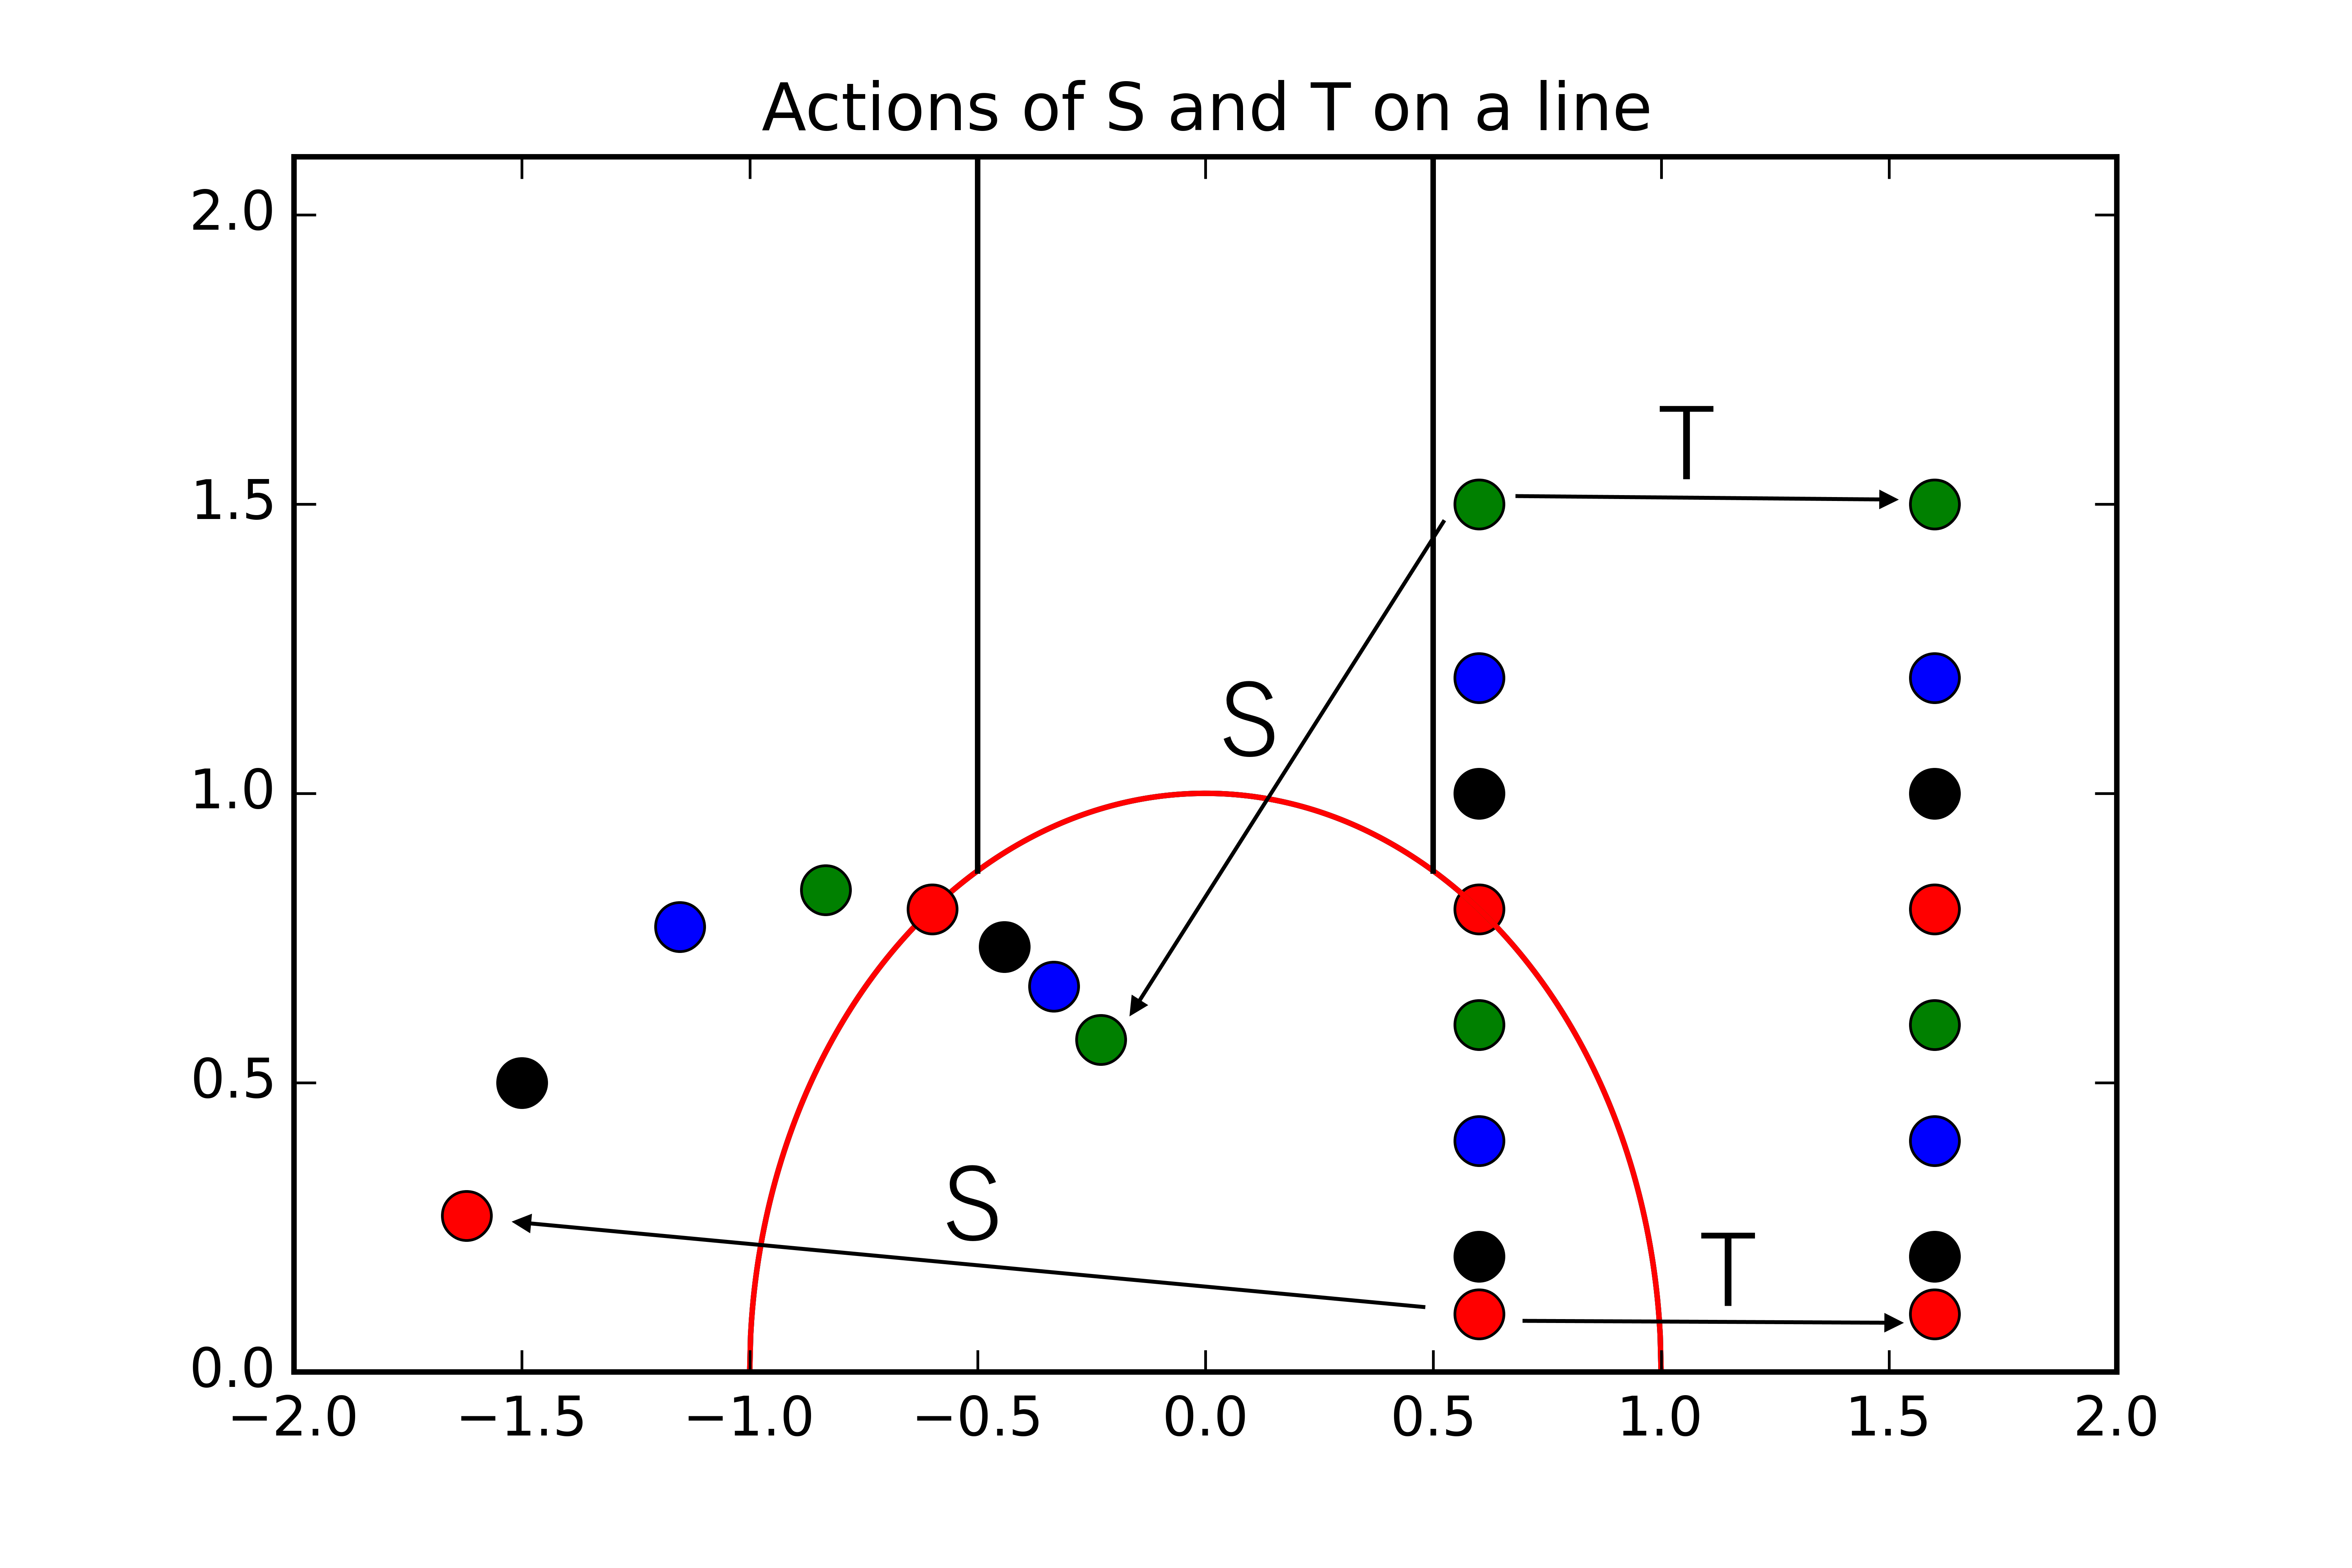
\includegraphics[height=2in]{ActionSTLine}
    \else
      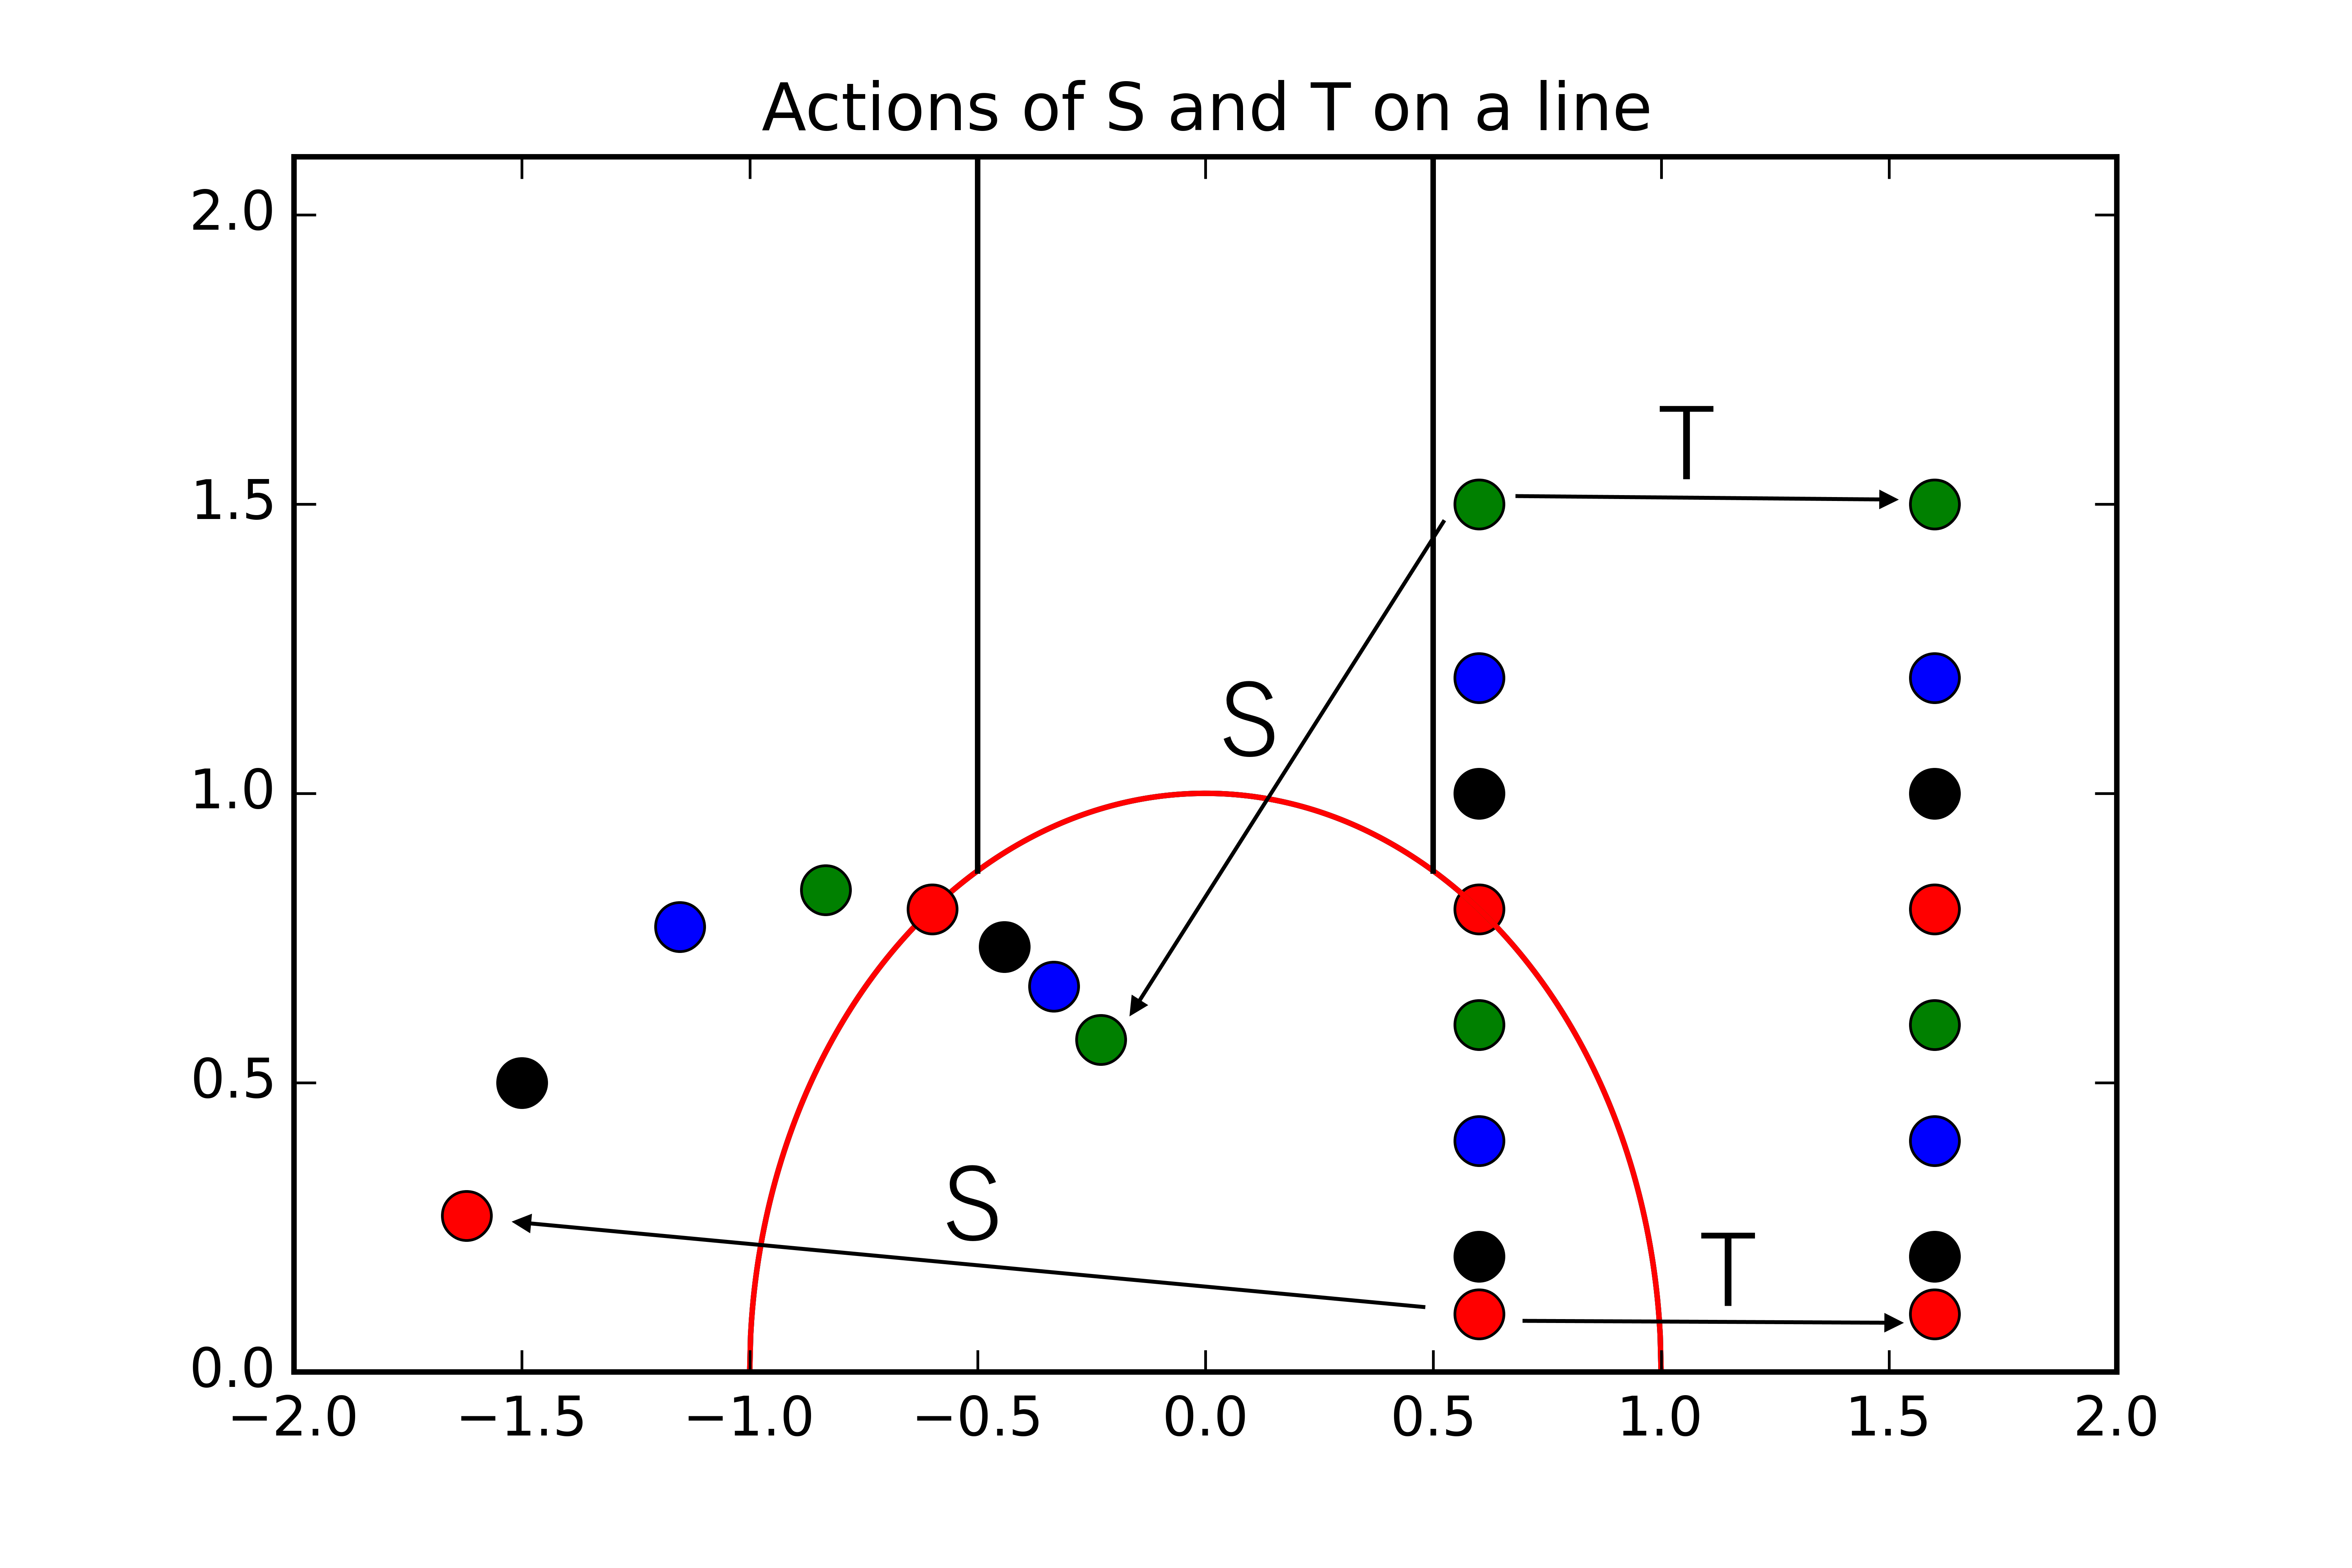
\includegraphics[bb = 92 86 545 742, height=6in]{ActionSTLine}
    \fi
    \caption{Example: action of $S$ and $T$}
    \label{fig:actionST}
  \end{center}
\end{figure}

\begin{figure}[!htbp]
\centering
\begin{subfigure}{.5\textwidth}
  \centering
      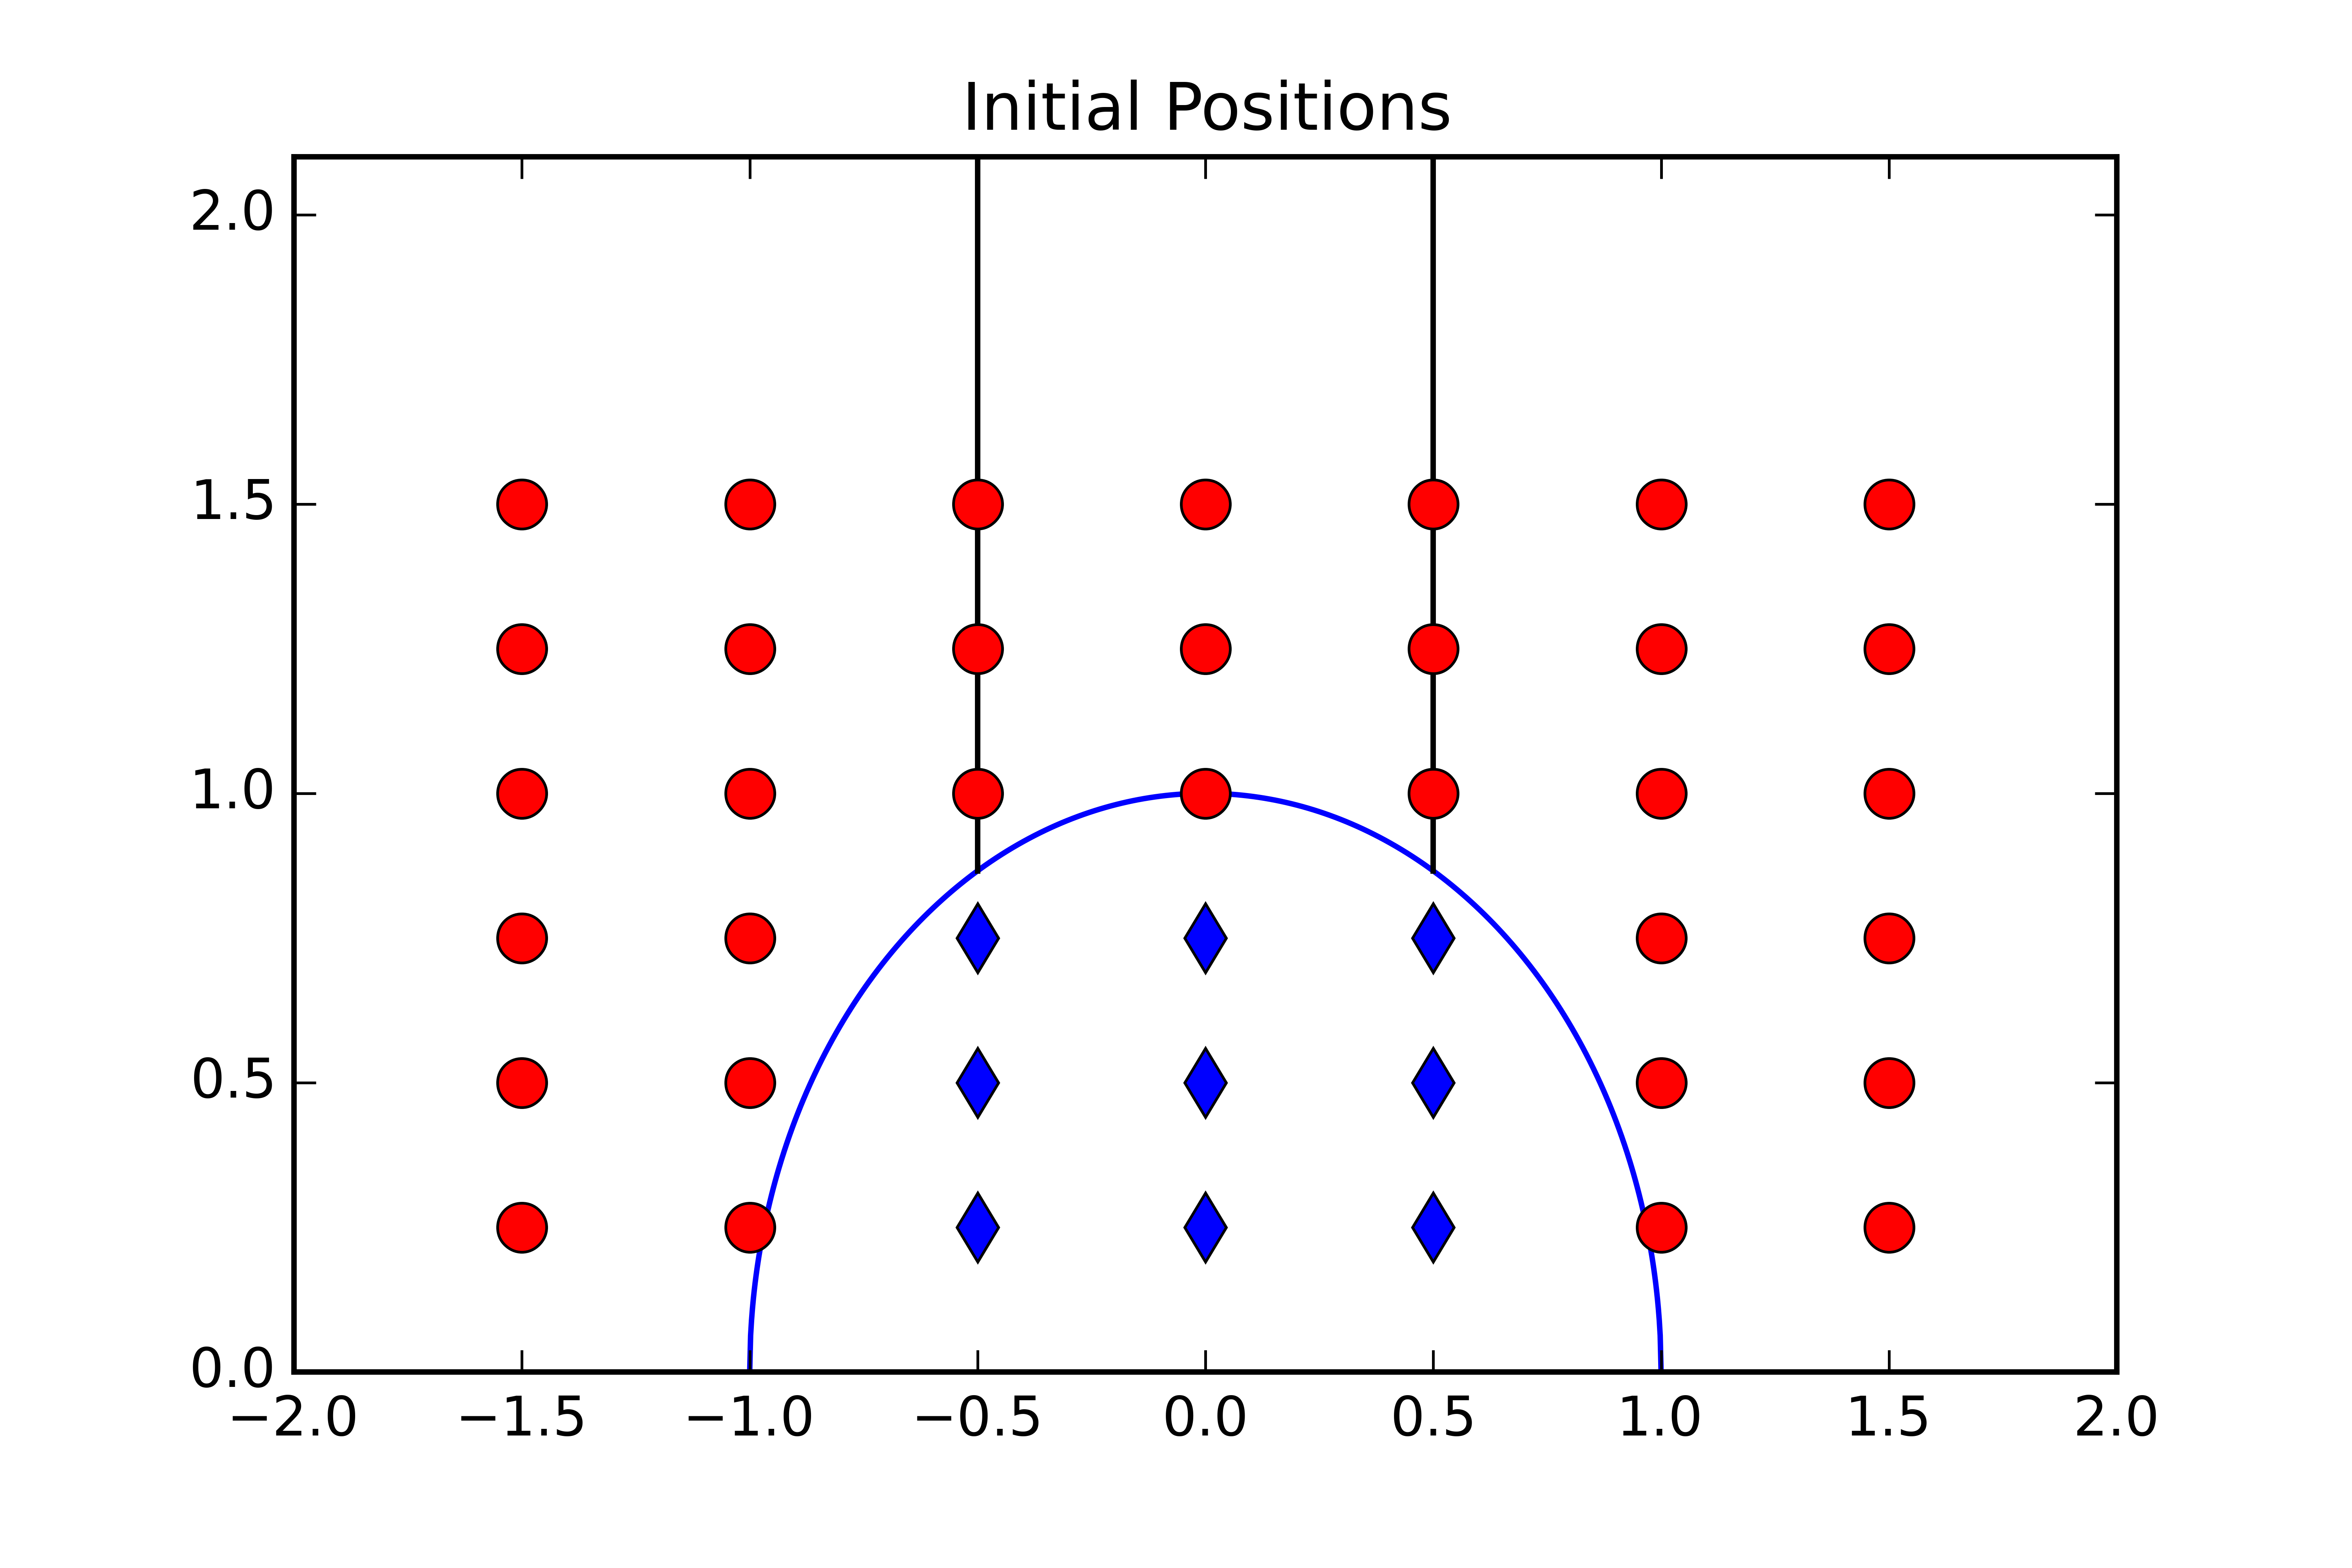
\includegraphics[height=2in]{SGridTransform-0}
  \caption{Before}
  \label{fig:beforeS}
\end{subfigure}%
\begin{subfigure}{.5\textwidth}
  \centering
      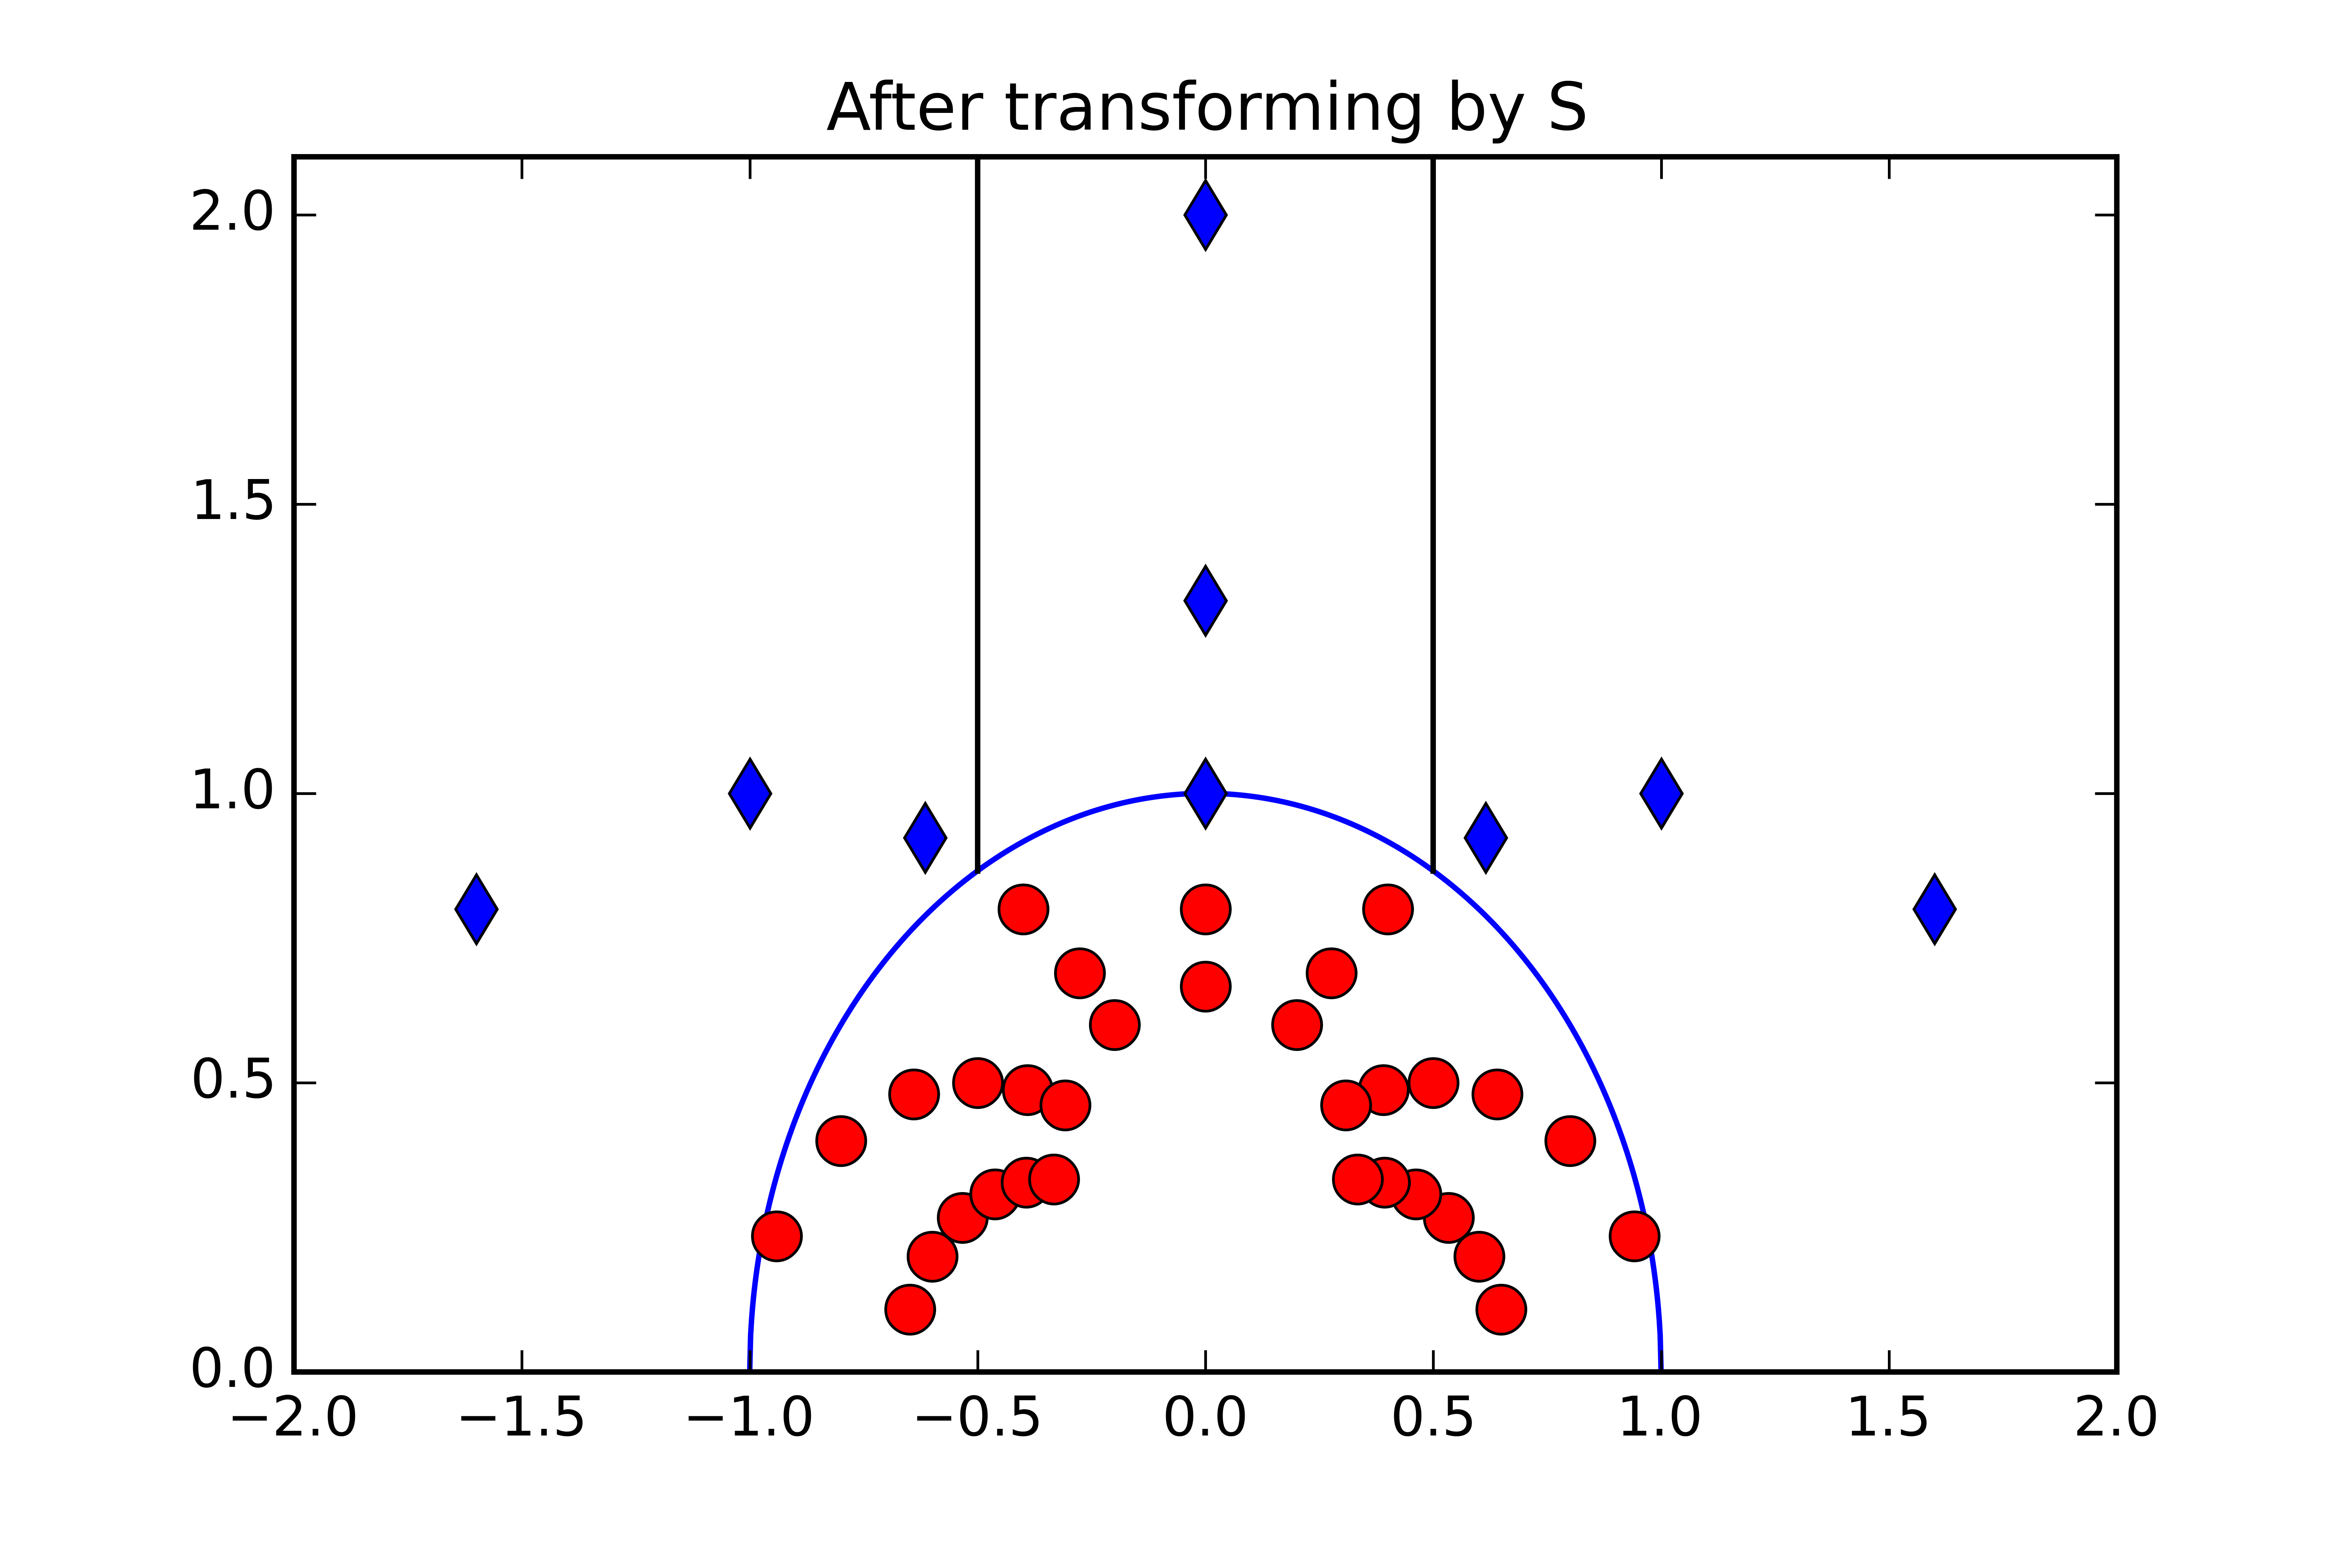
\includegraphics[height=2in]{SGridTransform-1}
  \caption{After action by $S$}
  \label{fig:afterS}
\end{subfigure}
\caption{Example: Action on grid of points }
\label{fig:actionS}
\end{figure}

We can define a group action of $\sltz$ on the upper half plane $\mathcal{H}$ through Möbius transformations. \\
Let $ A = \abcd \in \sltz$ and let $z \in \mathcal{H}$, we define the group action $A \cdot z = h(A)(z) = \frac{az +b}{cz +d}$.\\
We can check this satisfies the definition of group action given in \ref{def:groupAction}.
This group action satisfies associativity: if we have $A, B \in \sltz$, then for $z \in \mathcal{H}$, 
\begin{align*}
A \cdot (b \cdot z)  = A \cdot (h(B)(z)) & = h(A)(h(B)(z))  \\
 \quad & = (h(A)h \circ (B))(z)  \\
\small{(h \text{ is a homomorphism})} \quad \quad & = h(AB)(z) = (AB) \cdot z
\end{align*}

The second condition of being a group action is also satisfied, $I_2 \cdot (z) = z$ for all $z \in \mathcal{H}$.\\
\\


From now on we often refer to $\sltz$ as $\Gamma$. 

\begin{definition}
Let $\Gamma'$ be a subgroup of $\Gamma$. Two points $z_1, z_2$ in $\mathcal{H}$ are said to be $\Gamma'$ equivalent if they are in the same $\Gamma'$-orbit. That is to say there exists a $\gamma \in \Gamma'$ such that $\gamma z_1 = z_2$. 
\end{definition}
Note: Recall the notation $\gamma z$ for $\gamma \in \Gamma$ and $z \in \mathcal{H}$ means the group action of $\gamma$ on $z$, i.e $h(\gamma)(z)$. 
\begin{definition}
A fundamental domain $\mathcal{F}$ for a subgroup $\Gamma'$ of $\Gamma$ is a closed subset of $\mathcal{H}$ such that 
\begin{enumerate}
\item $ \cup_\gamma \Gamma' \gamma(\mathcal{F}) =\mathcal{H}$,
\item the images $\gamma(\text{int}(\mathcal{F}$)) are pairwise disjoint; that is $\gamma_1(\text{int}(\mathcal{F})) \cap \gamma_2(\text{int}(\mathcal{F})) = \emptyset$ if $ \gamma_1, \gamma_2 \in \Gamma', \gamma_1 \neq \gamma_2$. \\
( Here int($\mathcal{F}$) denotes the \textit{interior} of $F$, the largest open set contained inside $\mathcal{F}$ ). 
\end{enumerate}
\end{definition}

Restating the above definition gives, a closed subset of $\mathcal{H}$, $\mathcal{F}$, is a fundamental domain for $\Gamma'$ if 
\begin{enumerate}
\item The orbit of every $z \in \mathcal{H}$ contains some point in $\mathcal{F}$ 
\item No two distinct points in the interior of $\mathcal{F}$ are contained in the same orbit.
\end{enumerate}
We say that the images of $\mathcal{F}$ under $\Gamma'$ \textit{tessellate} $\mathcal{H}$.

\begin{example}\label{ex:fundamentalDomainT}
Consider the subgroup $\langle T \rangle$ of $\Gamma$, which has corresponding subgroup $\{\gamma_n \, \vert \, \gamma_n(z) = z+n, \, n \in \mathbb{Z}\}$ in $\mobh$ under the image $h \, : \, \Gamma \rightarrow \mobh$. The set $\mathcal{F} = \{ z \in \mathcal{H} \vert 0 \leq Re(z) \leq 1 \}$ is closed. Let $z \in \mathcal{H}$, then $ \leq n Re(z) < n+1$ for some $n \in \mathbb{N}$. We consider $Re(\gamma_{-n}(z)) = Re(z - n) = Re(z) - n$, which lies in the interval $ 0 \leq Re(\gamma_{-n}z) < 1$, so $\gamma_{-n}(z) \in \mathcal{F}$. \\
Next suppose we have $z_1, z_2 \in$ int($\mathcal{F}$), in particular $ 0 \leq Re(z_1) < Re(z_2) \leq 1$, and suppose $\gamma_n z_1 = z_2$ for some $n$. The bounds on $z_1$ and $z_2$ mean that the maximum distance is $1$ and so $\gamma_n = \gamma_1 = z + 1$. The only two points distance $1$ in the interval $[0,1]$ are $0$ and $1$, so $Re(z_1) = 0$ and $Re(z_2) = 1$. So they do not lie in the interior of $\mathcal{F}$. \\
Hence $\mathcal{F}$ is a fundamental domain for $\langle T \rangle$. 



\end{example}

\begin{example}\label{ex:fundamentalDomainS}
The set $\mathcal{F} = \{z \in \mathcal{H} \, \vert \, \vert c \vert \leq 1\}$ is a fundamental domain for the group $\Gamma' = \langle S \rangle$. The subgroup of $\mobh$ corresponding to $\Gamma'$ is $\{z, -1/z\}$.\\
Let $z$ be a point in $\mathcal{H}$ that is not in $\mathcal{F}$, then $-1/z$ is in the fundamental domain. \\
If $z_1, z_1$ are two distinct $\Gamma'$ equivalent points then we must have $-1/z_1 = z_2$, this occurs only when $\vert z_1 \vert = \vert z_2 \vert = 1$, i.e only on the boundary of $\mathcal{F}$.
\end{example}


\subsection{Geometric proof that $S,T$ generate $\sltz$}

The geometric proof of Theorem \ref{thm:STGenerateSLTZ} is done in two main steps. First we construct a fundamental domain for $\Gamma$ using the action of $G: = \langle S, T \rangle \subset \Gamma$, next we use it to show $G \supset \Gamma$ and so $G = \Gamma$. 
\\ 
The actions of $S, T$, along with the fundamental domains of $\langle T \rangle$ and $\langle S \rangle$ give an idea of one possible fundamental domain for $\Gamma$.

\begin{lemma}\label{lem:gorbitfund}
Every element $z\in \mathcal{H}$ has an element of it's G-orbit in $\mathcal{F} = \{z \in \mathcal{H} \, | \, -1/2 \leq z \leq 1/2 \, |z| \geq 1  \}$.
\end{lemma}
(Note: This implies every element of $Z \in \mathcal{H}$ has an element of it's $\Gamma$-orbit in $\mathcal{F}$, since $G \subset \Gamma$).

\begin{proof}

Let $g  = \abcd \in G$, let $z \in \mathcal{H}$. Then as we've observed in \ref{eqn:imaginaryMobius},
$$ Im(gz) = \frac{Im(z)}{{\vert cz +d \vert}^2}.$$
Geometrically since $c,d$ are integers the points $cz+d$ lie on the lattice generated by $1$ and $z$. 
This means that there is no infinite decreasing sequence 
$$\vert c_1z + d_1  \vert > \vert c_2z + d_2  \vert > \vert c_3z + d_3  \vert  > \cdots  \text{ for integers } c_i,d_i.$$ 
This is since for any $\lambda \in \mathbb{R}, c \in \mathbb{Z}$ we could find $d$ sufficiently large such that $\vert cz + d \vert > \lambda$ and $\vert cz -d \vert > \lambda$. So given $c \in \mathbb{Z}$ there are finitely many $d_i \in \mathbb{Z}$ such that $\vert cz + d_i \vert < \vert c_1z + d_1  \vert$. For each such $d_i$ there are finitely many $c_i$ that satisfy $\vert cz + d_i \vert < \vert c_1z + d_1  \vert$. Thus the sequence is finite and must terminate.
\\
It implies there is no infinite increasing sequence 
$$ Im(g_1z)  < Im(g_2z) < \cdots \text{ for } g_i\in G$$

This means that the following procedure will eventually move every element $z$ in $\mathcal{H}$ in to the fundamental domain $\mathcal{F}$.\\
Let $z = z_0$.
\begin{enumerate}[(i)]
\item Translate $z_0$ to $z_1$ by $T^n$ such that $| Re(T^nz)| \leq 1/2$ for some $n \in \mathbb{N}$. ( We showed this was possible, for a translated domain, in Example \ref{ex:fundamentalDomainT}).
\item If $z_1$ lies in the fundamental domain we are done. If not then it must lie inside the unit circle with $|z_1| < 1$, so we invert by $S$ to get $z_2 = S(z_1)$. Observe that 
$$ Im(z_2) = Im(Sz_1) = \frac{Im(z_1)}{{|z_1|}^2} > Im(z_1) \text{ since } |z_1| < 1.$$
\item If $z_2$ is in the fundamental domain we are done, otherwise let $z_0 = z_2$ and return to the first step.
\end{enumerate}
From this procedure we get a sequence 
$$Im(z) < Im(ST^{n_1}z) < Im(ST^{n_2}ST^{n_1}z) < \cdots,$$
we noted already that such a sequence must be finite, so eventually the process will terminate.
\end{proof}

An example of this procedure applied to multiple points is given in Figure \ref{fig:procedure}.
\begin{figure}[!htbp]
\begin{tabular}{cc}
  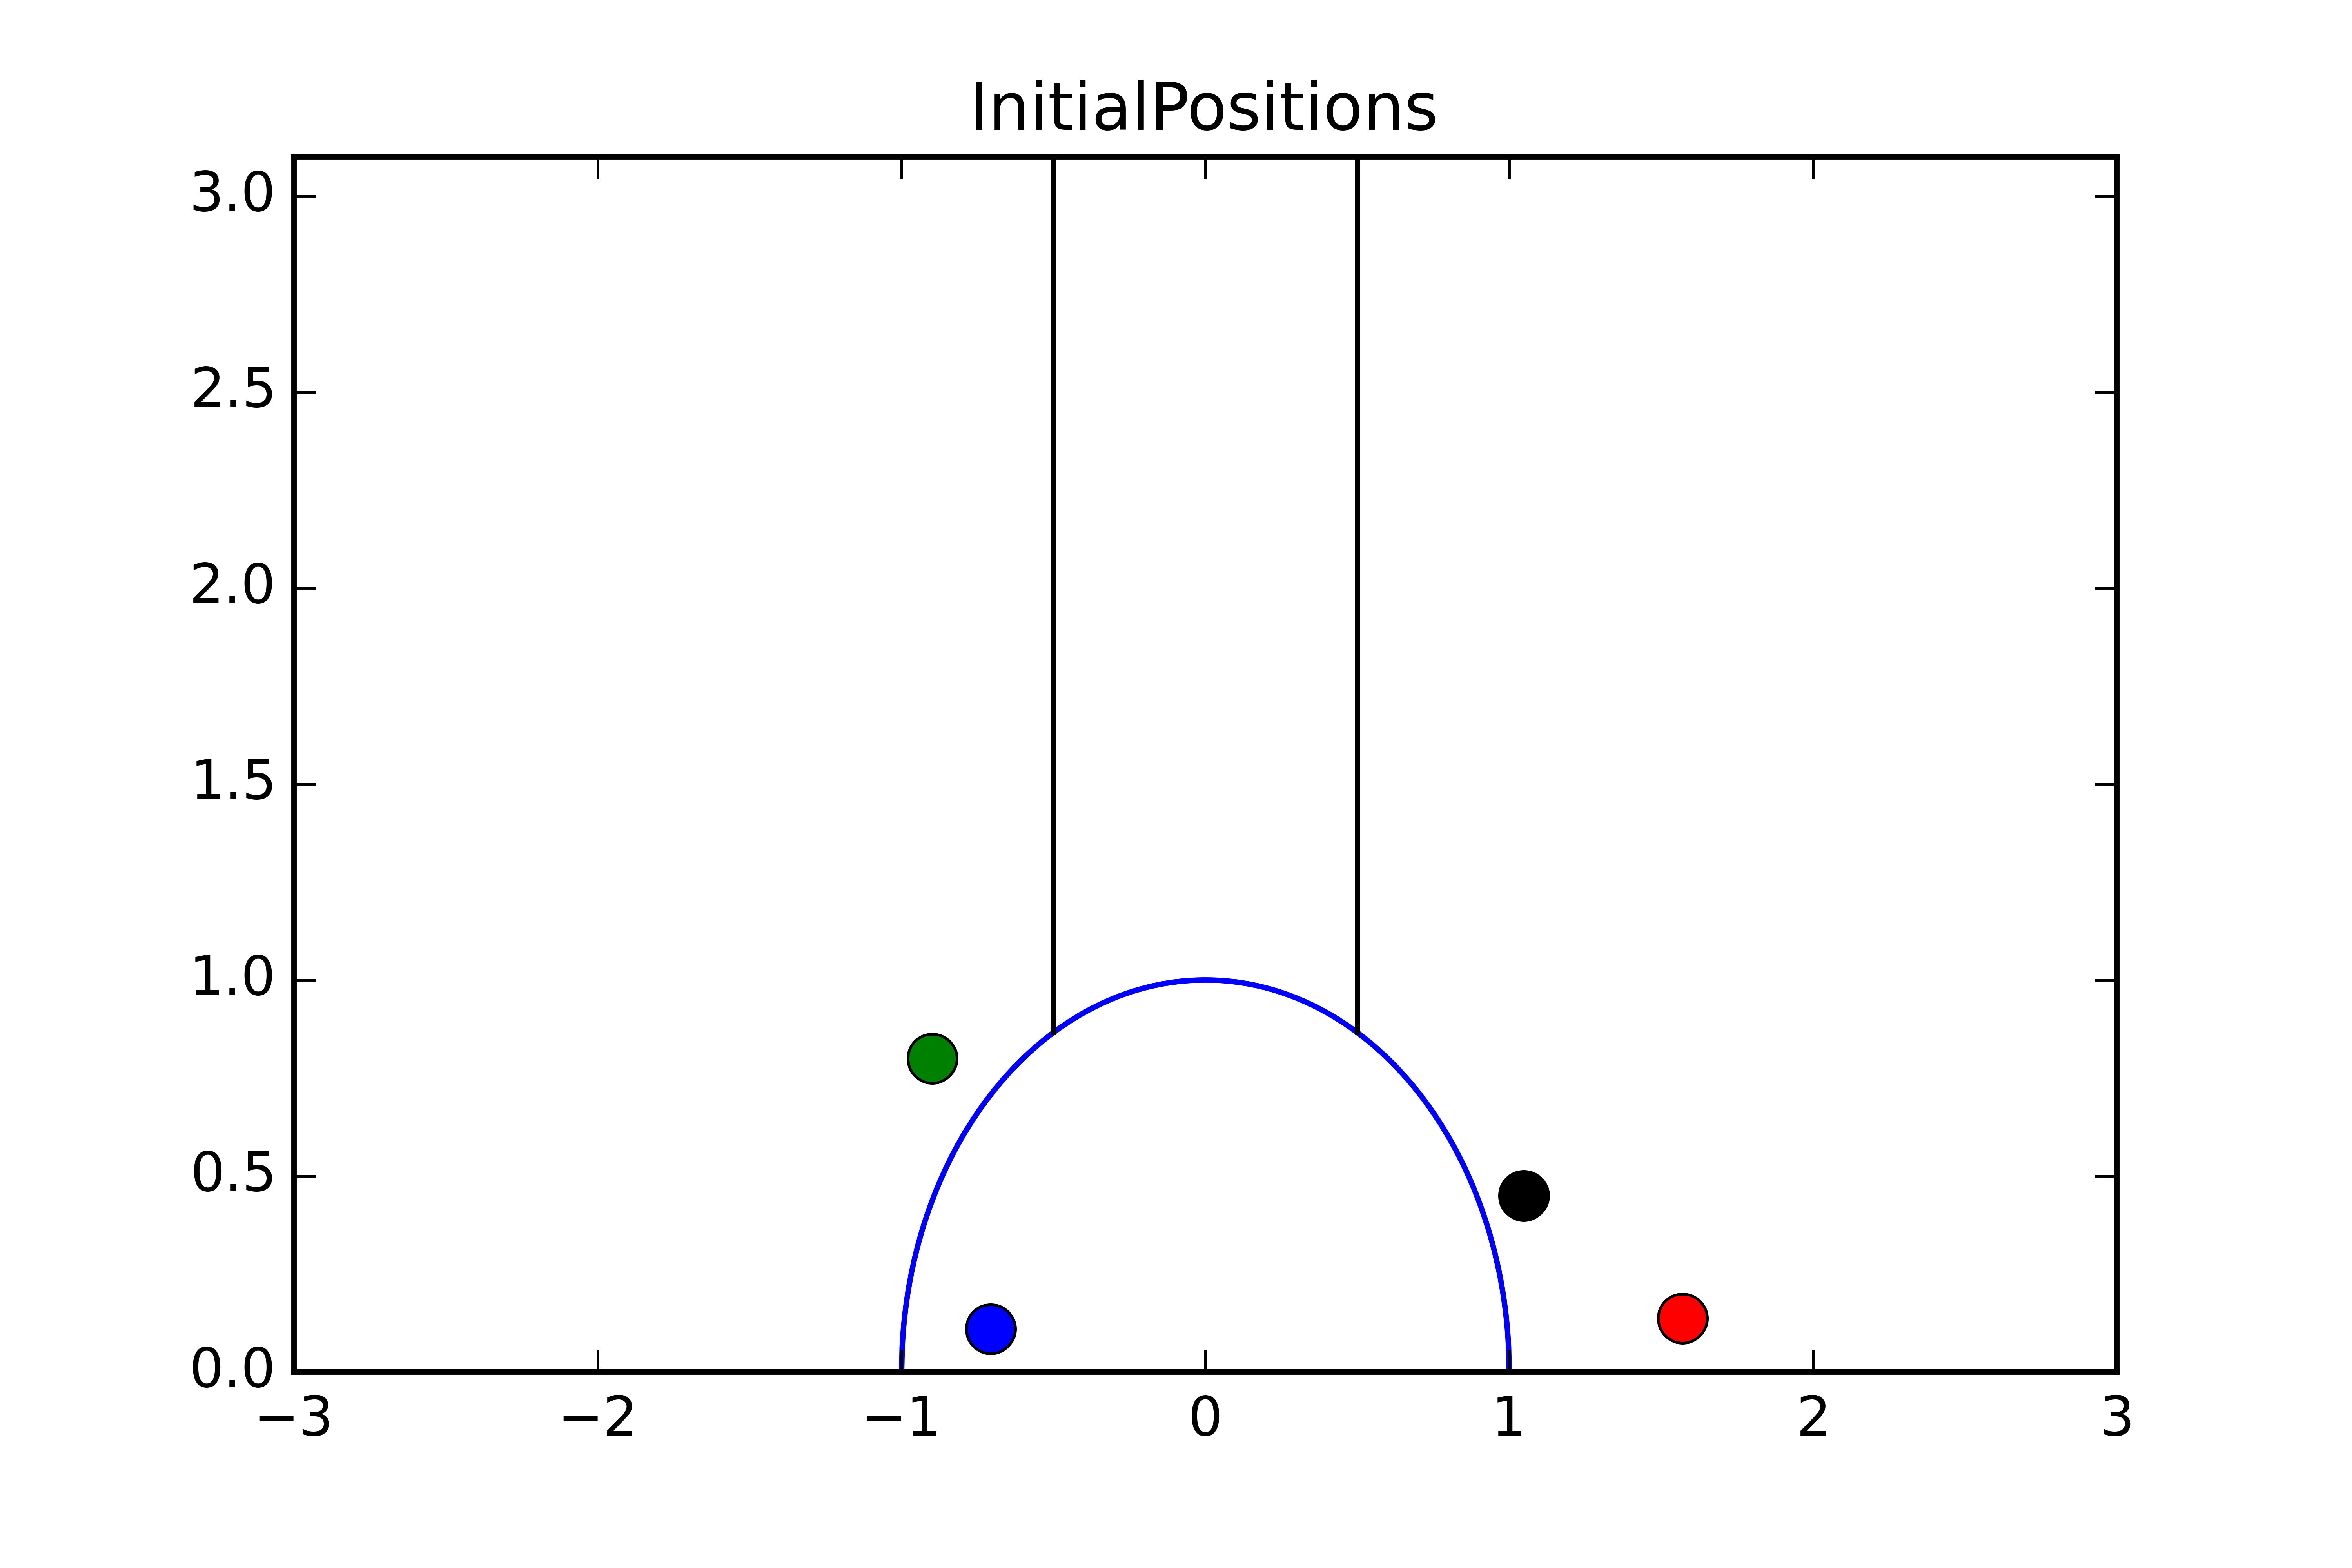
\includegraphics[width=65mm]{FundDomain-0} &   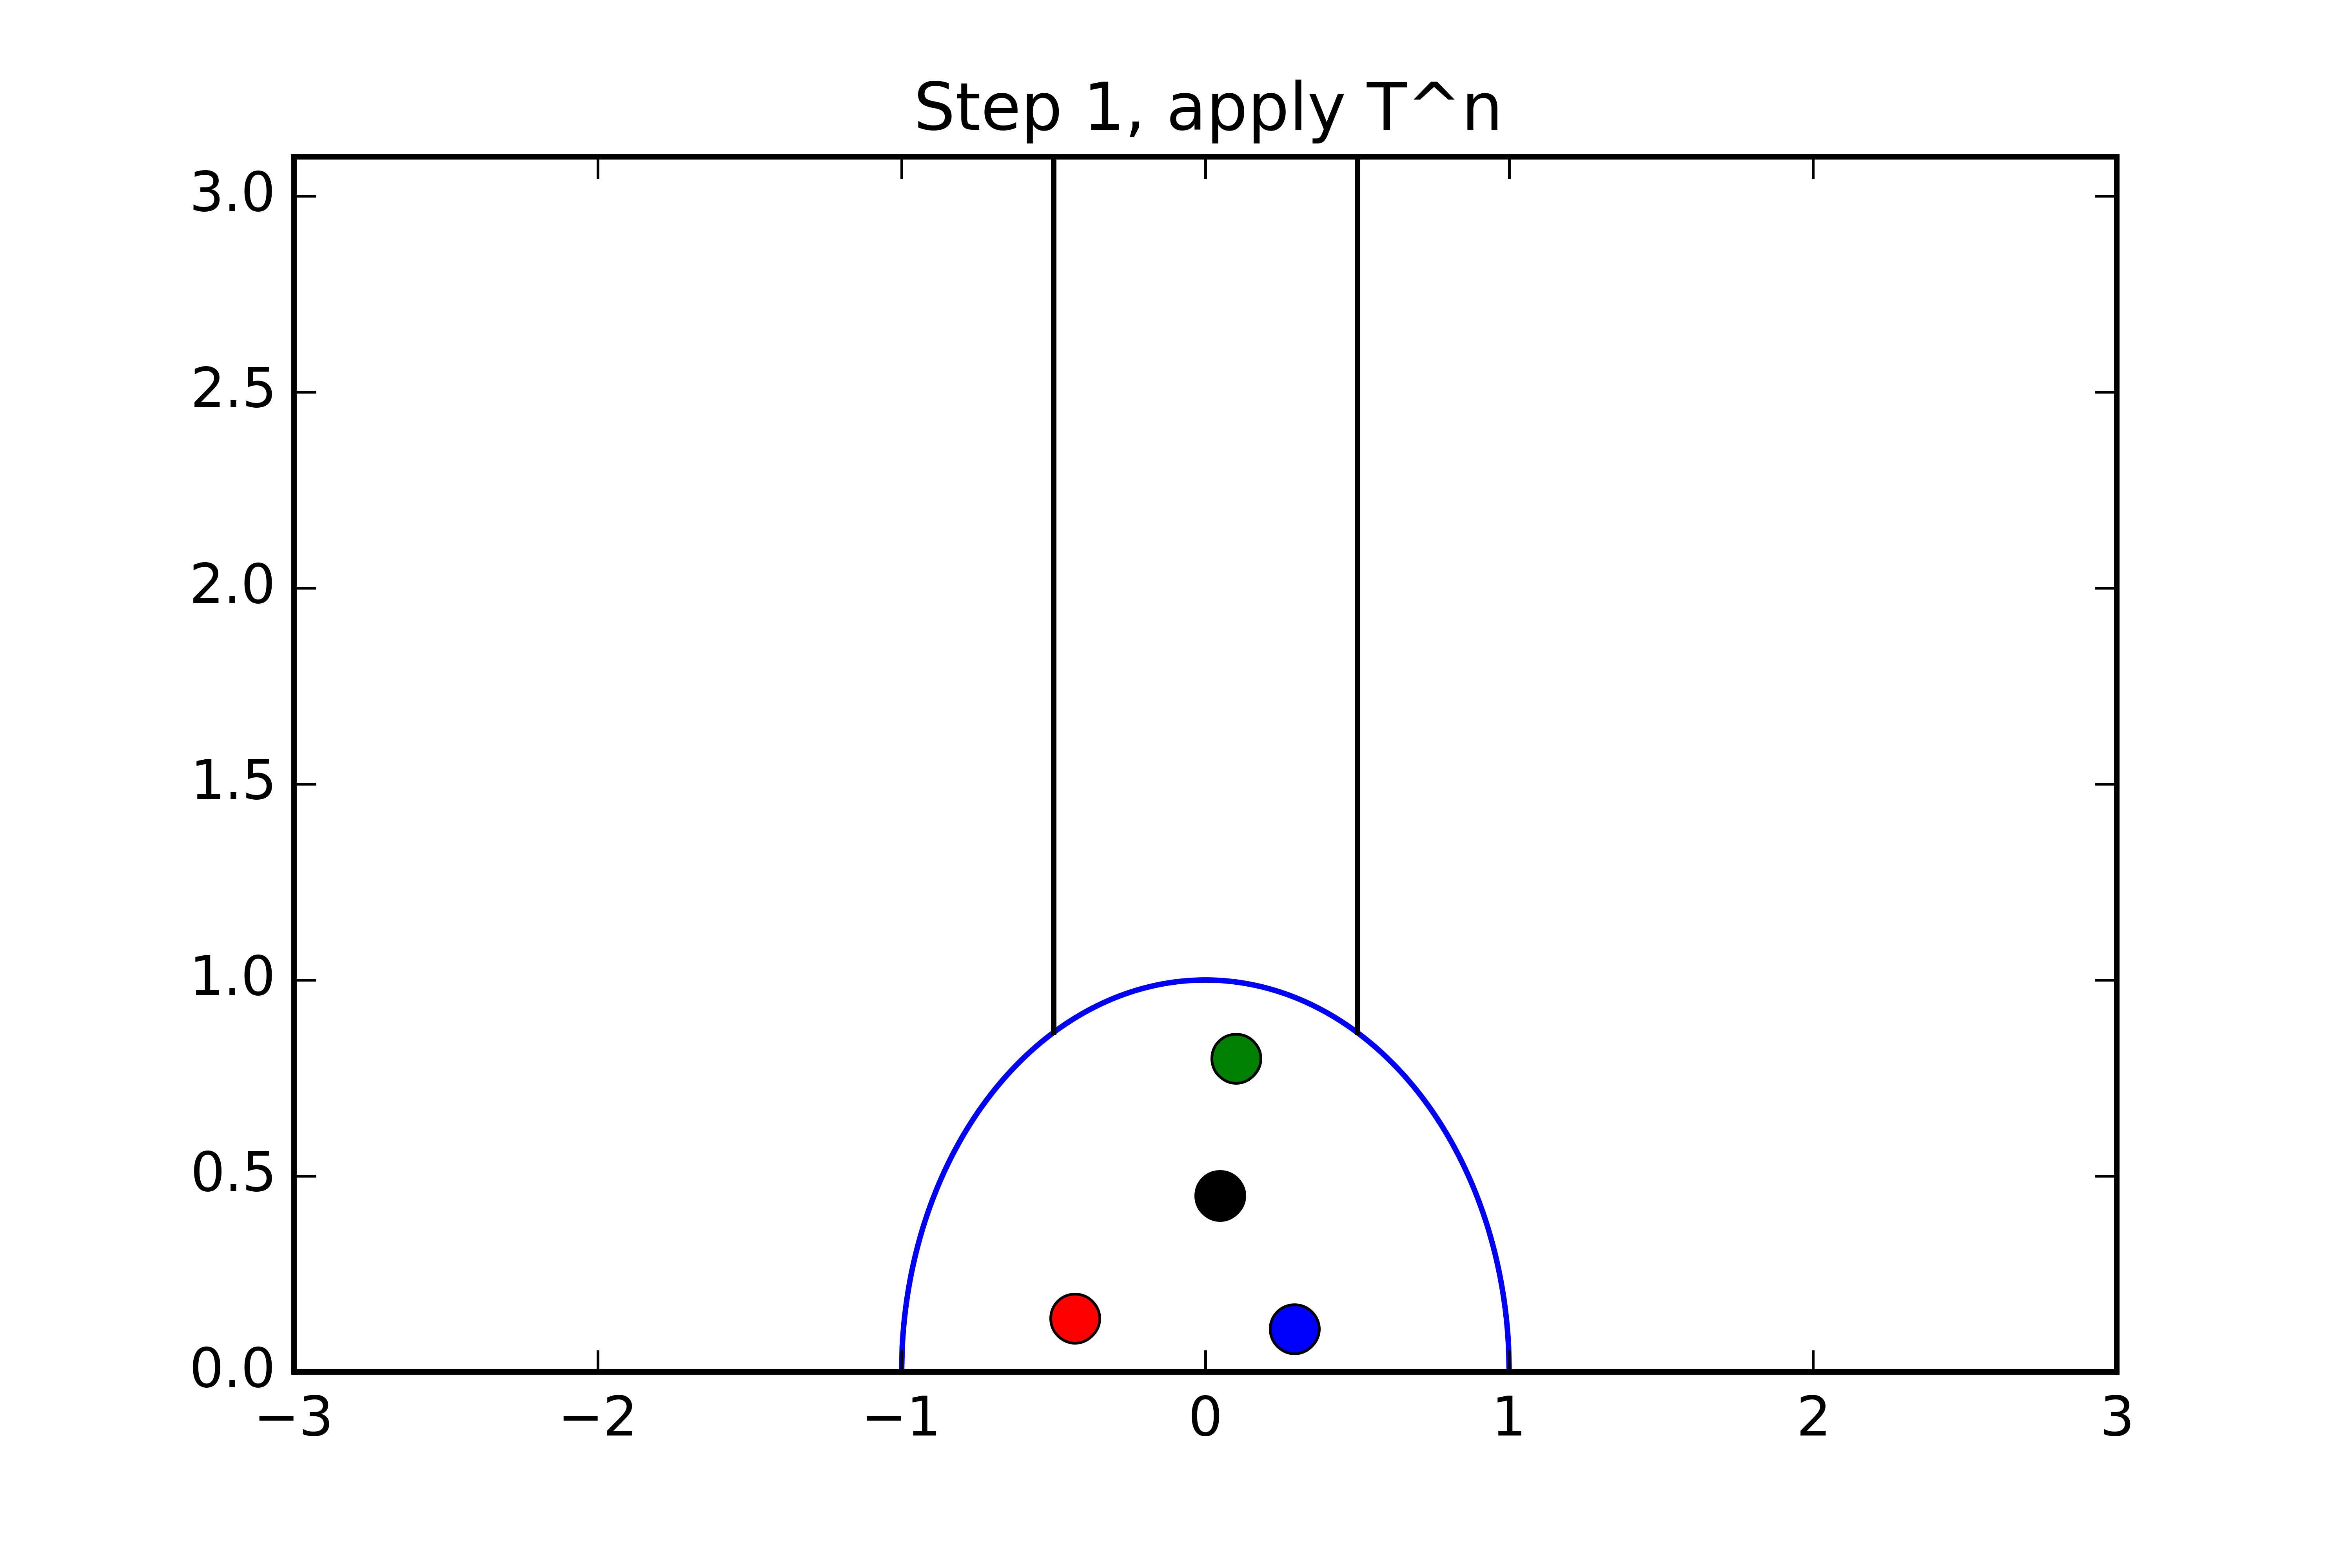
\includegraphics[width=65mm]{FundDomain-1} \\
(a) Initial & (b) Apply $T^n$ \\[6pt]
 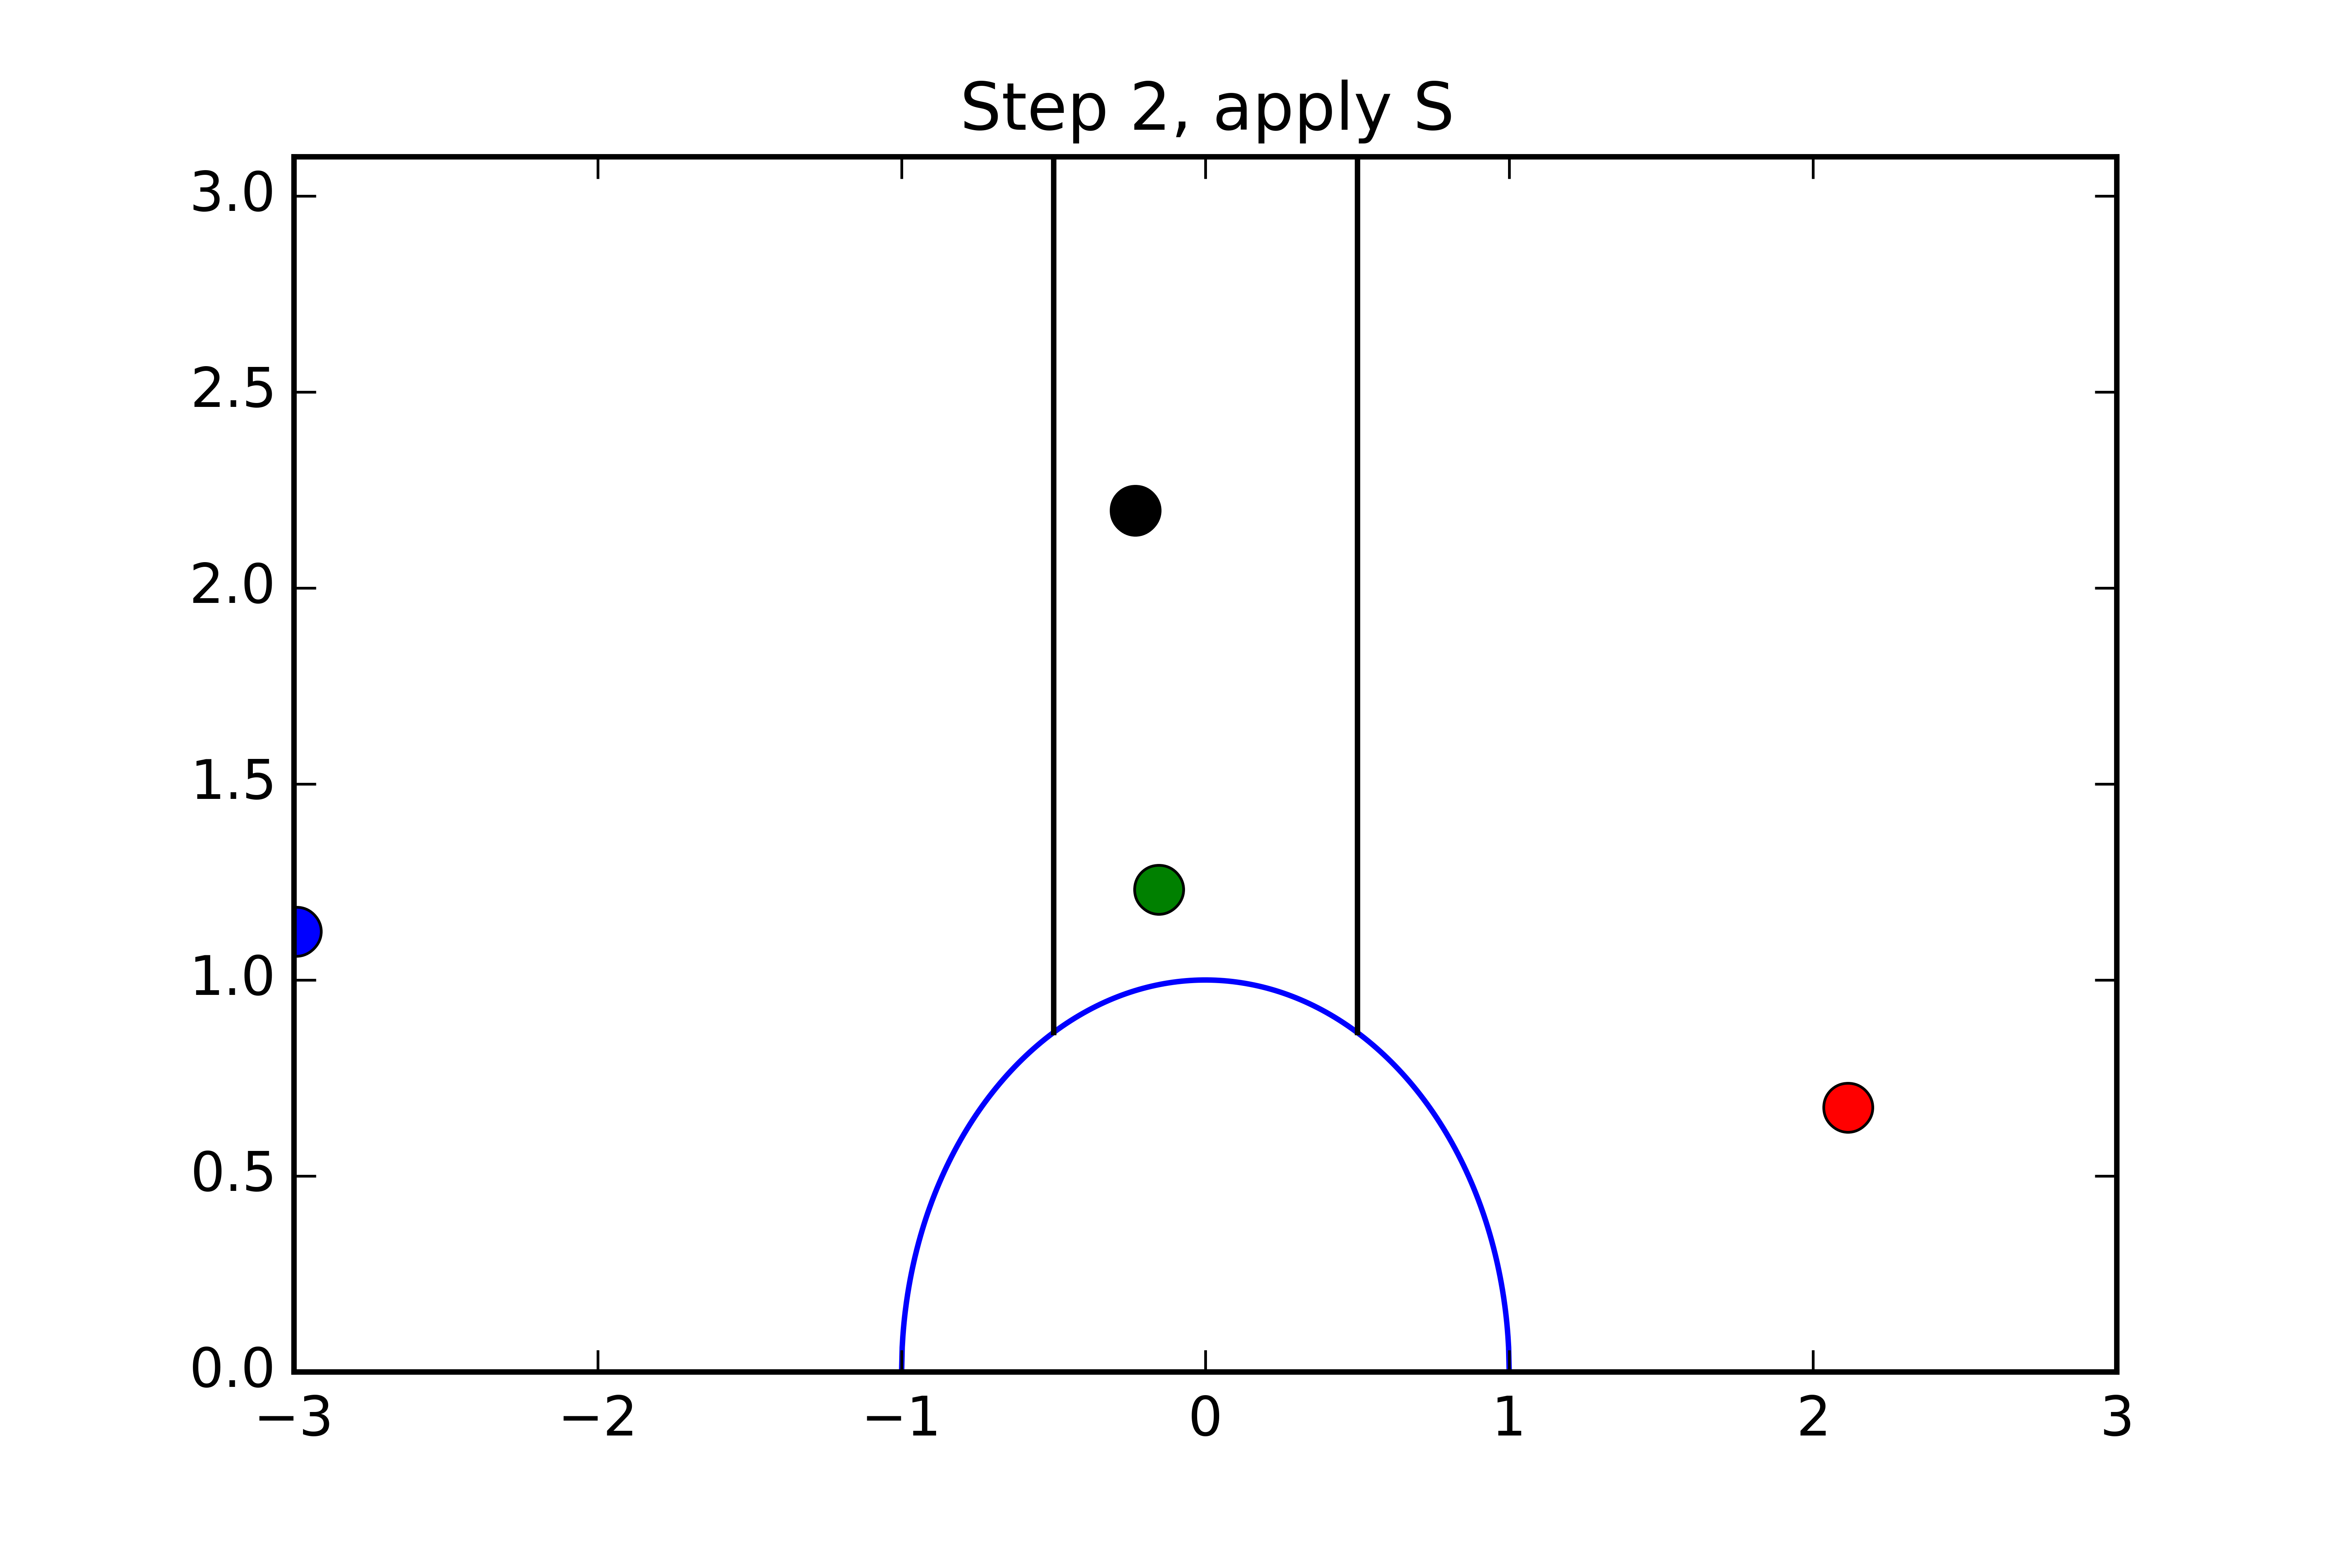
\includegraphics[width=65mm]{FundDomain-2} &   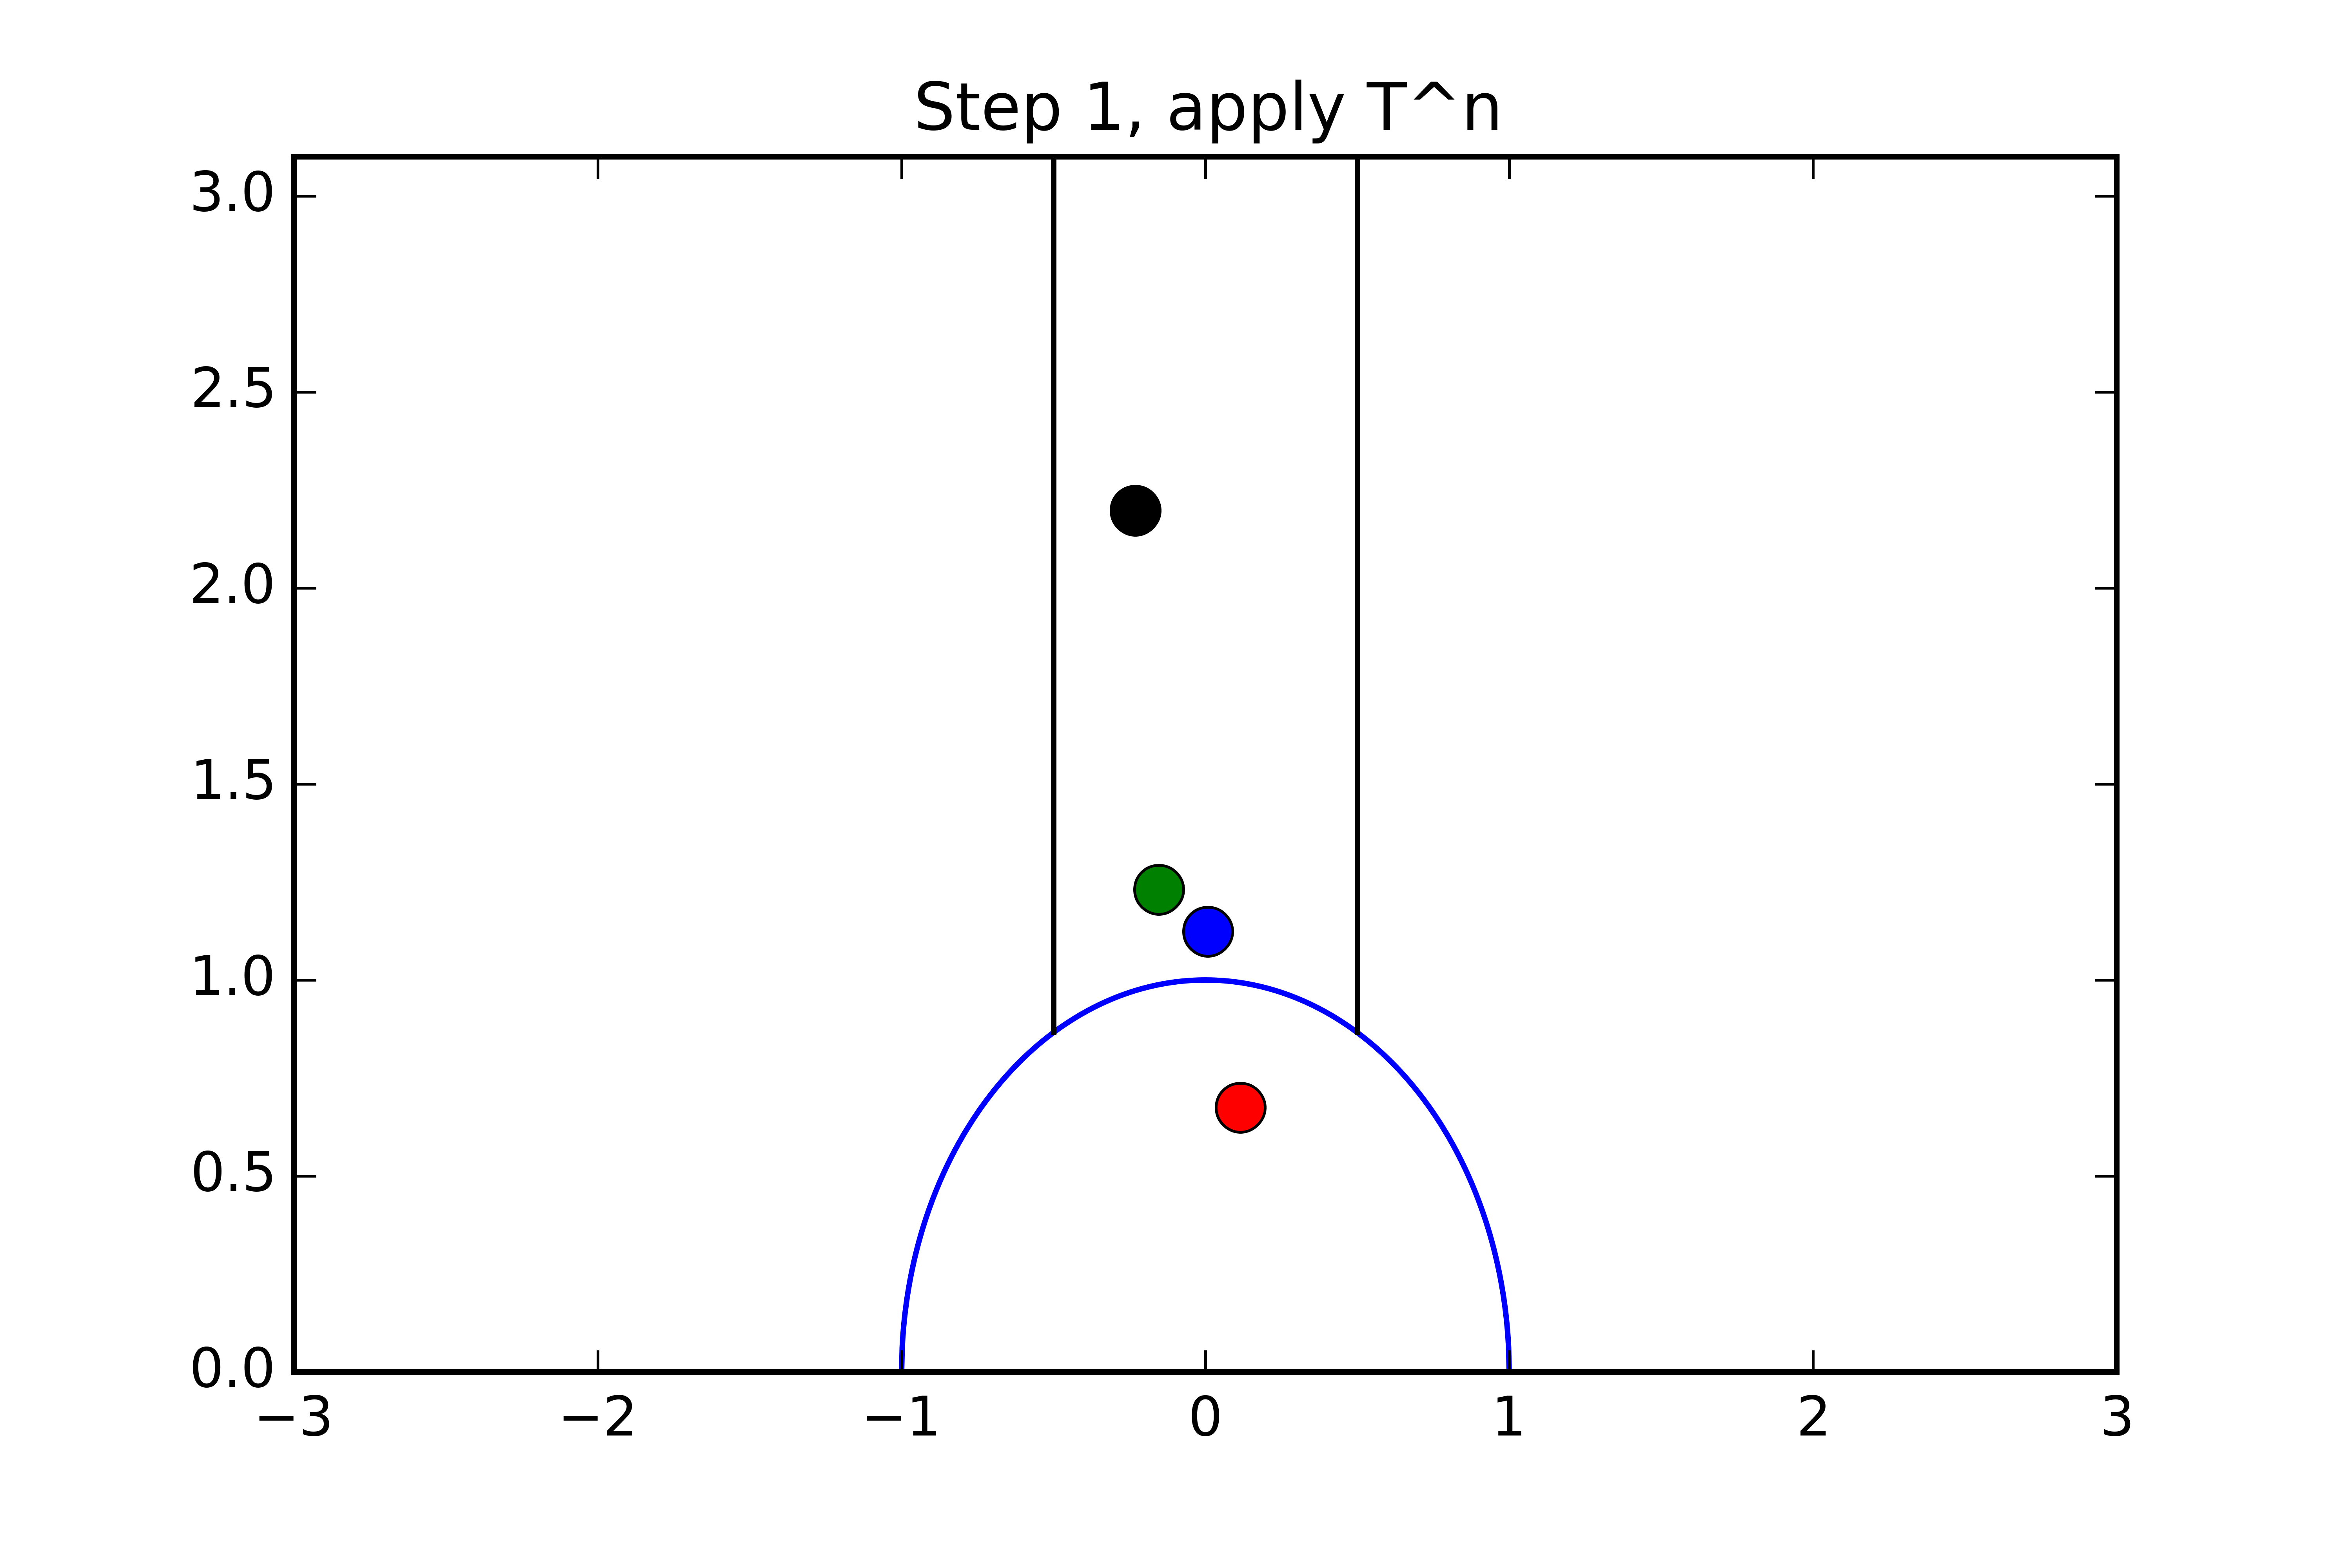
\includegraphics[width=65mm]{FundDomain-3} \\
(c) Apply S & (d) Apply $T^n$  \\[6pt]
\multicolumn{2}{c}{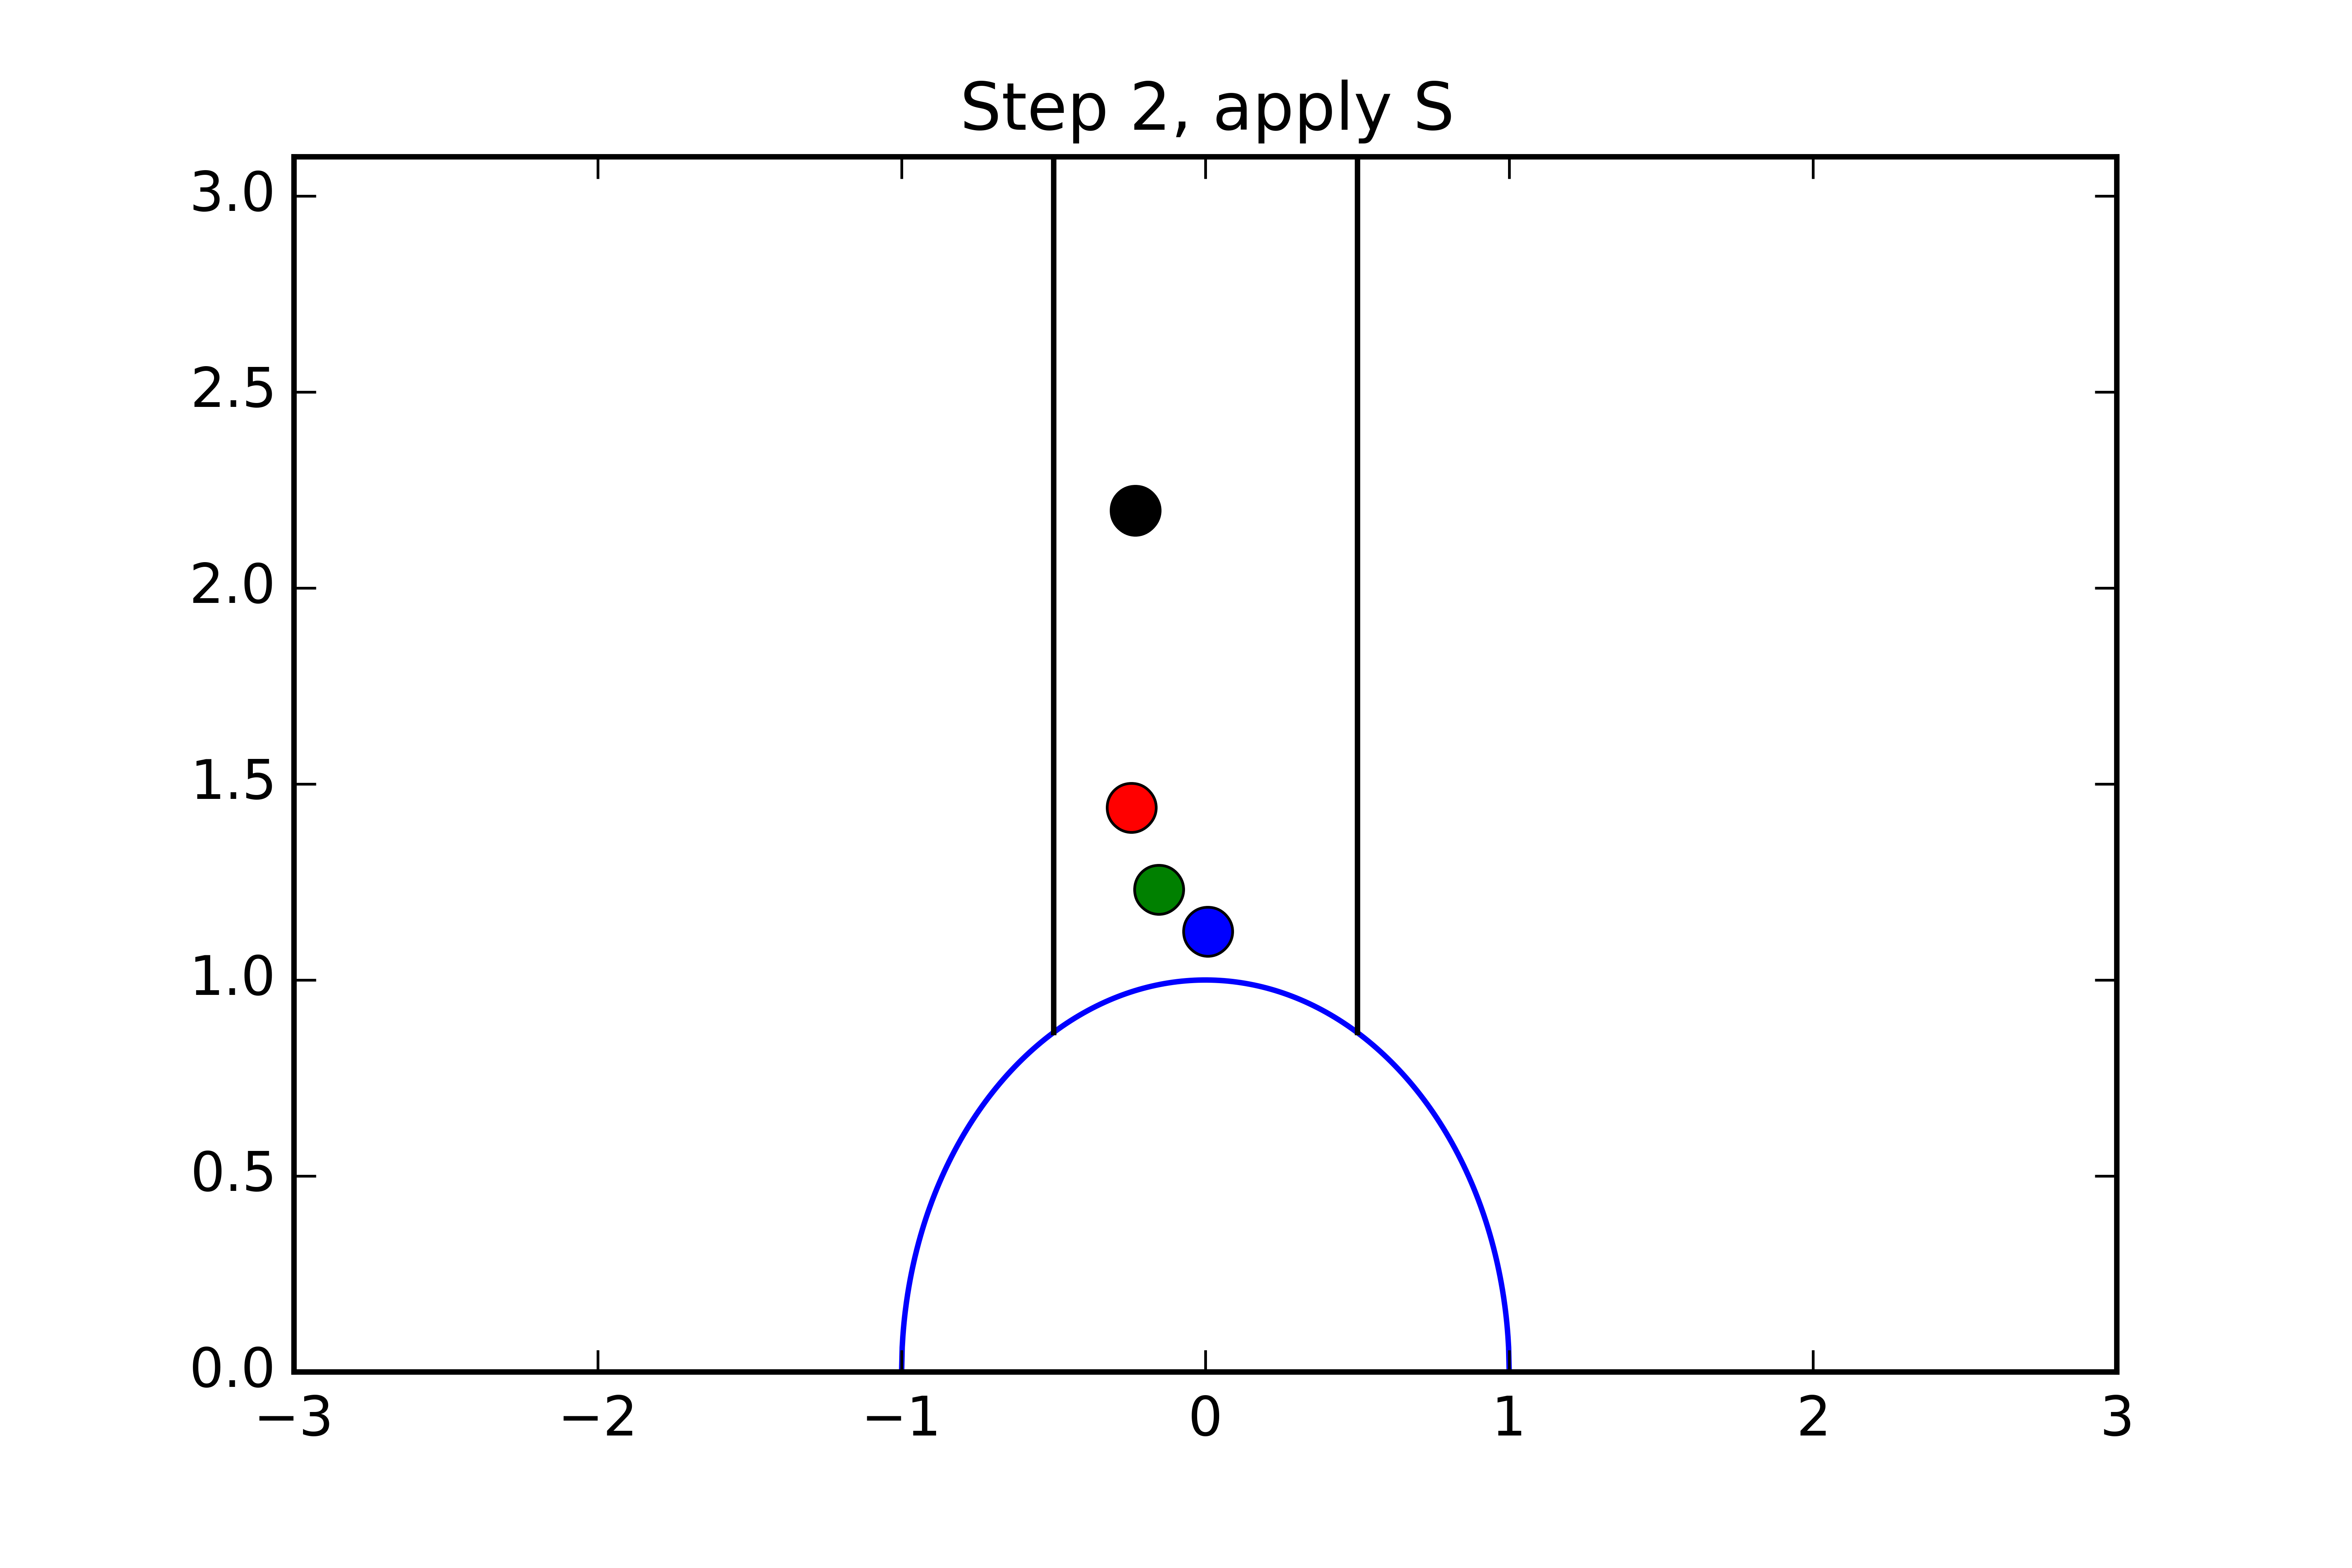
\includegraphics[width=65mm]{FundDomain-4} }\\
\multicolumn{2}{c}{(e) Apply $S$}
\end{tabular}
\caption{Example of procedure given in Lemma \ref{lem:gorbitfund} . }
\label{fig:procedure}

\end{figure}

\begin{lemma}\label{lem:noDistinctInteriorEquiv}
No two distinct points in the interior of $\mathcal{F}$ are $\Gamma$-equivalent
\end{lemma}

\begin{proof}

Suppose we have two distinct points $z_1, z_2 \in \mathcal{F}$ and there exists a $\gamma  = \abcd \in \Gamma$ such that $\gamma z_1 = z_2$. I.e $ -1/2 \leq Re(z_1), Re(z_2) \leq 1/2$ and $|z_1|, |z_2| \geq 1$.  We will show that both the points must lie on the boundary of $\mathcal{F}$. \\
Assume without loss of generality that $Im(z_1) \leq Im(z_2)$($\star$). \\
Writing out $Im(z_2)$ explicitly using \ref{eqn:imaginaryMobius}, 
\begin{align}
Im(z_2) = Im(\gamma z_1) &= \frac{Im(z_1)}{{|cz_1 +d |}^2} \overset{(\star)}{\geq} Im(z_1) \nonumber\\
& \implies |cz_1 + d | \leq 1 \label{eqn:boundCZD}
\end{align}
We will now investigate the possible values for $c,d$ based on the bound $|cz_1 +d | \leq 1$. The values we find for $c,d$ along with the condition on the determinant $ad -bc$ = 1 will allow us to determine all the possible matrices $\gamma$.\\
\\
If $|c| \geq 2$ then $Im(cz_1) \geq 2Im(z_1) \overset{Im(z_1) \geq 1}{\geq} \sqrt{3}$ and so $Im(cz_1 +d) > 1$. The imaginary part of $cz_1 +d$ thus lies outside the unit circle, it follows that the point $cz_1 +d$ lies outside the unit circle and so $|cz_1 +d| > 1$, which is a contradiction to \ref{eqn:boundCZD}. \\
The simplifies the possible $c,d$ pairs greatly since we must have $c \in  \{-1,0, 1\}$. \\
We consider the following cases separately, 
\begin{enumerate}[(i)]
\item $c = 0$: \\
Here the condition on the determinant means $ad = 1$ and so $a = d = \pm 1$. Thus $\gamma = \pm \left(\begin{array}{ c c } 1 & \pm b \\ 0 & 1 \end{array} \right)$, and so $\gamma = \pm T^{\pm b}$. \\
If $b = 0$ then $\gamma \pm I_2$ and so $\gamma z_1 = z_1$, which is a contradiction. \\
If $b \neq 0$, then $|Re(\gamma z_1)| = |Re(z_1) \pm b| \geq |Re(z_1) \pm 1| \geq  1/2$. So $\gamma z_1$ is only in $\mathcal{F}$ if $|Re(\gamma z_1)| = 1/2$, i.e only if $b = \pm 1$ and $\gamma = \pm T^{\pm 1}$. So $z_2 = z_1 \pm 1$, therefore they both lie on the boundary. 

\item $c = \pm 1$, $d = 0$: \\
The condition on the determinant gives $-bc = 1$ and so $c = -b = \pm 1$. Then $\gamma = \pm \left(\begin{array}{ c c } \pm a &  -1 \\ 1 & 0 \end{array} \right)$ thus it is of the form $\gamma = \pm T^{\pm a}S$. \\

The inequality \ref{eqn:boundCZD} gives $|\pm z_1 | = |z_1| \leq 1$, so $z_1$ since $z_1 \in \mathcal{F}$ we have $|z_1| = 1$. So $|Sz_1| = |-1/z_1| =1$. We are thus in the situation of (i) where we consider $-1/z_1$ instead of $z_1$, and $a$ in place of $b$. It follows that if $a = 0$, that $-1/z_1 = z_1$ and so $z_1^2 = -1$, the only solution in $\mathcal{H}$ is $z_1 = i$ and so $z_1= z_2$ and lies on the boundary of $\mathcal{H}$. \\
If $a \neq 0$ it follows from (i) that the only solution is $a = \pm 1$, and $-1/z_1 \pm 1 = z_1$. So the two possibilities are $z_1 = z_2 = \frac{1}{2} + i \frac{\sqrt{3}}{2}$ where $\gamma = \pm TS$ or $z_1 = z_2 = -\frac{1}{2} + i \frac{\sqrt{3}}{2}$ where $\gamma = \pm T^{-1}S$. These are the two points that lie both on the unit circle and one of the lines $Re(z)= \pm 1/2$. 

\item $c = \pm 1$, $d \neq 0$: \\
The inequality \ref{eqn:boundCZD} gives the condition $ |\pm z_1 +d | \leq 1$. But since $\mathcal{F}$ is symmetric this is equivalent to $|z_1 + d |\leq 1$. We can write it out fully as $|z_1 + d| = \sqrt{(x +d)^2 + y^2}$ where $z = x + iy$, firstly it's clear $|z_1 + d| \geq   \sqrt{(x +d)^2} = |(x +d)|$, since $y^2 > 0$. Suppose $|d| \geq 2$, then use $ -1/2 \leq x \leq 1/2$ to get $|x+d| \geq -1/2 +d$. Therefore $|\pm z_1 + d| \geq 3/2 > 1$ for $|d| \geq 2$, which is a contradiction. \\
So the only other possibility is $d = \pm 1$, We can repeat the above but include that the minimum value for $y$ is $\frac{\sqrt{3}}{2}$ and use the fact that $(x \pm 1)^2 \geq 1/4$ , so $|z_1 \pm 1| =\sqrt{(x \pm 1)^2 + y^2} \geq \sqrt{1/4 + 3/4} = 1$. Thus we must have 
$$|\pm z_1 \pm 1| = 1.$$
From this we go through all the possibilities: \\
Let $\omega^+ = \frac{1}{2} + i \frac{\sqrt{3}}{2}, \omega^- = -\frac{1}{2} + i \frac{\sqrt{3}}{2}$.
\begin{itemize}

\item Case, $c = d = 1$ : \\
Then $ |z_1 + 1| =1 \implies  z_1 = \omega^- $. The determinant of $\gamma$ is $a -b  =1 \implies a = b +1$. This means $\gamma =  \left(\begin{array}{ c c } b+1 &  b \\ 1 & 1 \end{array} \right)= T^{b+1}ST$, note $ST(z_1) = z_1$. \\
If $b = 0$, then $\gamma = \left(\begin{array}{ c c } 1 &  0 \\ 1 & 1 \end{array} \right) = TST$ and $\gamma z_1 =\omega^+$.\\
If $b = -1$ then $\gamma = \left(\begin{array}{ c c } 0 & -1 \\ 1 & 1 \end{array} \right) = ST$, $\gamma z_1 = z_1$.\\
For any other value of $b$ then $\gamma z_1$ will not lie in the fundamental domain.

\item Case, $c = -d = 1$ : \\
Then $|z_1 -1 | = 1 \implies z_1 = \omega^+$. The determinant of $\gamma$ is $ -a -b =1 \implies a = 1-b$. This means $\gamma =  \left(\begin{array}{ c c } 1-b &  b \\ 1 & -1 \end{array} \right) =  T^{-b}STS$, note $ STS(z_1) = \omega^-$. \\
If $b = 0$, then $\gamma = \left(\begin{array}{ c c } -1 &  0 \\ 1 & -1 \end{array} \right) = STS$ and $\gamma z_1 = \omega^-$.\\
If $b =-1$, then $\gamma = \left(\begin{array}{ c c } 0 &  -1 \\ 1 & 1 \end{array} \right) = (TS)^2$, and $\gamma z_1 = z_1$.\\
For any other value of $b$ then $\gamma z_1$ will not lie in the fundamental domain.

\item Case, $c = d = -1$ : \\
Then $|-z_1 - 1| = |z_1 +1| = 1  \implies z_1 = \omega^-$. The determinant of $\gamma$ is $-a + b =1 \implies a = b-1$. This means $\gamma =  \left(\begin{array}{ c c } b-1 &  b \\ -1 & -1 \end{array} \right) = -T^{-b}TST$, note $TST(z_1) = \omega^+$. \\
If $b = 0$, then $\gamma = \left(\begin{array}{ c c } -1 &  0 \\ -1 & -1 \end{array} \right) = -TST$, and $\gamma z_1 = \omega^+$. \\
If $b = 1$, the n $\gamma =  \left(\begin{array}{ c c } 0 &  1 \\ -1 & -1 \end{array} \right) = -ST$, and $\gamma z_1 = z_1$.

\item Case, $c = -d = -1$ : \\
Then $|-z_1 + 1| =1 \implies z_1 = \omega^+$. The determinant of $\gamma$ is $a +b =1 \implies a = 1-b$. This means $\gamma =  \left(\begin{array}{ c c } 1-b &  b \\ -1 & 1 \end{array} \right) = -T^{b}STS$, note $ STS(z_1) = \omega^-$. \\
If $ b = 0$, then $\gamma = \left(\begin{array}{ c c } 1 &  0 \\ -1 & 1 \end{array} \right) = STS$, and $\gamma z_1 = \omega^-$.\\
If $ b = 1$, then $\gamma = \left(\begin{array}{ c c } 0 &  1 \\ -1 & 1 \end{array} \right) = (TS)^2$, and $\gamma z_1 = z_1$

\end{itemize}

\end{enumerate}
\end{proof}

\begin{proposition}\label{prop:fundamentalDomain}
$\mathcal{F} = \{z \in \mathcal{H} \, | \, -1/2 \leq z \leq 1/2 \, |z| \geq 1  \}$ is a fundamental domain for $\Gamma$.
\end{proposition}
\begin{proof}
By applying Lemmas \ref{lem:gorbitfund} and \ref{lem:noDistinctInteriorEquiv} we see that $\mathcal{F}$ satisfies both parts of the definition for a fundamental domain. 
\end{proof}

\begin{figure}[!htbp]
  \begin{center}
    \leavevmode
    \ifpdf
      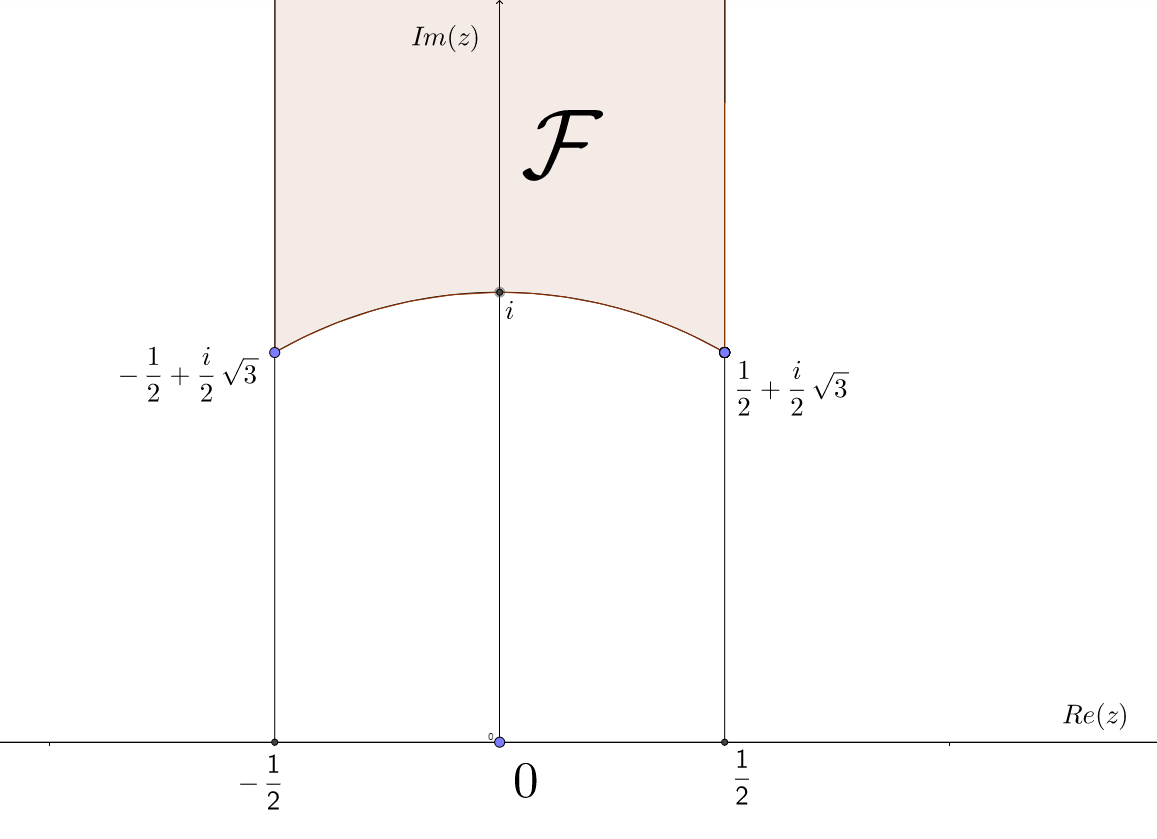
\includegraphics[height=3in]{FundamentalDomainGamma}
    \else
      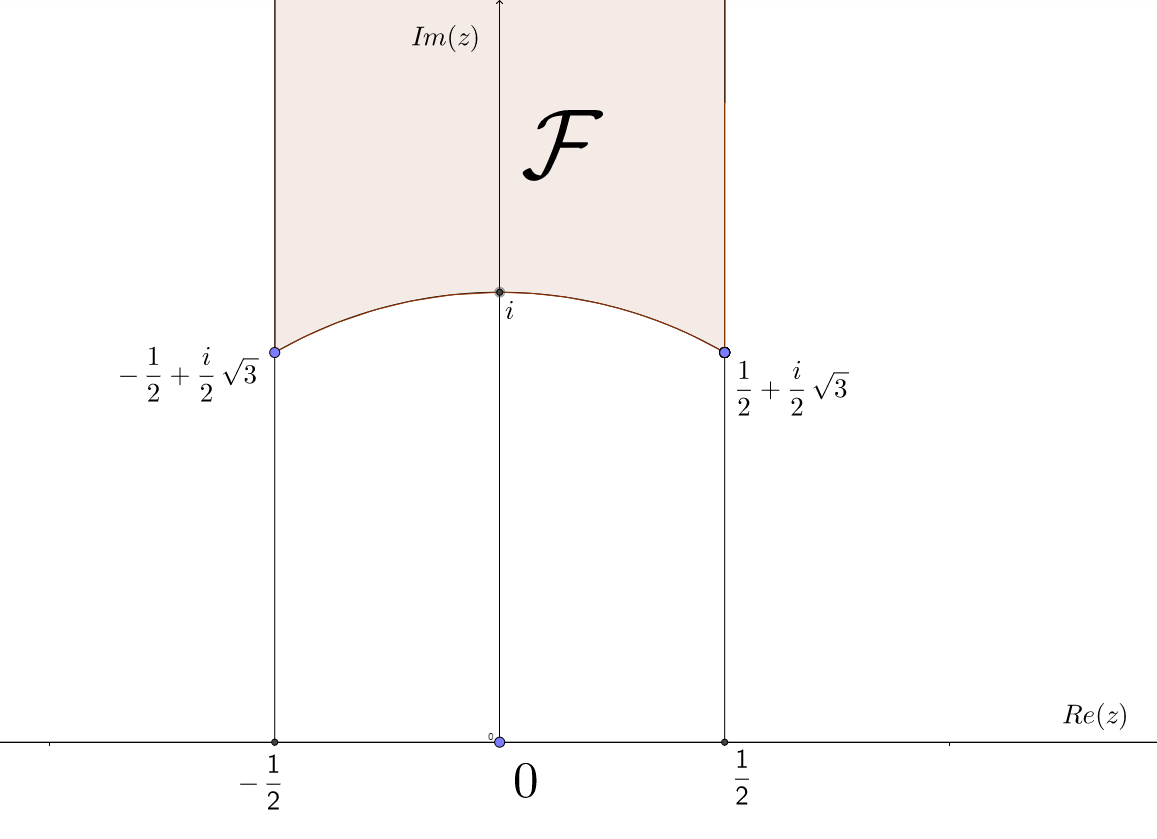
\includegraphics[bb = 92 86 545 742, height=6in]{FundamentalDomainGamma}
    \fi
    \caption{A fundamental domain $\mathcal{F}$ of $\Gamma$}
    \label{fig:fundDomainGamma}
  \end{center}
\end{figure}


See \ref{fig:kleinTessellation} for a tessellation of $\mathcal{H}$ by Klein \citep{klein}.

\begin{figure}[!htbp]
  \begin{center}
    \leavevmode
    \ifpdf
      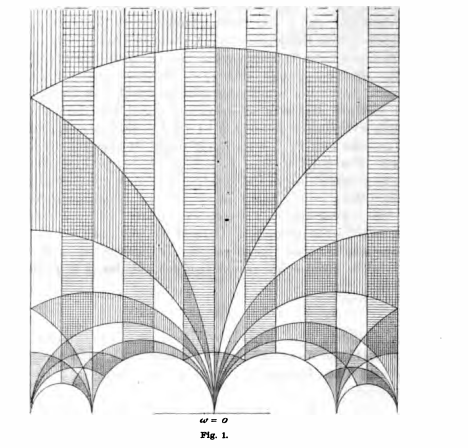
\includegraphics[height=3in]{KleinFundamentalDomain}
    \else
      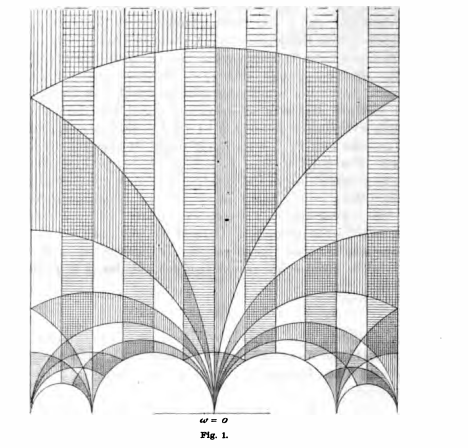
\includegraphics[bb = 92 86 545 742, height=6in]{KleinFundamentalDomain}
    \fi
    \caption{Tessellation of $\mathcal{H}$}
    \label{fig:kleinTessellation}
  \end{center}
\end{figure}


In the course of proving Lemma \ref{lem:noDistinctInteriorEquiv} we proved following two facts.
\begin{proposition}\label{prop:gammaEquivBoundary}
Two distinct points $z_1,z_2$ on the boundary of $\mathcal{F}$ are $\Gamma$-equivalent only if $Re(z_1) = \pm 1/2$ and $z_2 = z_1 \mp 1$ or $|z_1| =1$ and $z_2 = -1/{z_1}$
\end{proposition}

\begin{proposition}\label{prop:stabilizerGamma}
If $z \in \mathcal{F}$ then the stabilizer of $z$ in $\Gamma$, $\Gamma_z$, is $\{I,-I\}$, except in the following cases: \\
(i)   $\Gamma_z= \pm \{I,S\}$ if $z=i$\\
(ii)  $\Gamma_z= \pm \{I,ST, {(ST)}^2\}$ if $z=-1/2 + \frac{\sqrt{-3}}{2}$\\
(iii) $\Gamma_z= \pm \{I,TS, {(TS)}^2\}$ if $z=1/2 + \frac{\sqrt{-3}}{2}$\\
\end{proposition}


\begin{theorem}\label{thm:STGenerateSLTZGeometric}
The matrices $S,T$ generate $\Gamma$, i.e $\langle S, T \rangle =\sltz$.
\end{theorem}
\begin{proof}
Let $\gamma$ be an element of $\Gamma$, and let $z$ be a point in the interior of $\mathcal{F}$. Then consider the point $\gamma z \in \mathcal{H}$. In lemma \ref{lem:gorbitfund} we showed that there exists a $g \in \langle S, T \rangle$ such that $g \gamma z \in \mathcal{F}$. So the points $z$ and $g\gamma z$ are $\Gamma$ equivalent. 
But since $z$ is in the interior of $\mathcal{F}$ it follows from Propositions \ref{prop:fundamentalDomain} and \ref{prop:stabilizerGamma} that $g \gamma = \pm I_2$ and so $\gamma = g^{-1} \in \langle S, T \rangle$.
\end{proof}

The proof of Theorem \ref{thm:STGenerateSLTZGeometric} can be used to write an element $\gamma \in \Gamma$ as a word in $S, T$. Take a point in int($\mathcal{F}$), like $2i$, then consider the point $\gamma 2i$. We use the algorithm described the proof of Lemma \ref{lem:gorbitfund} to find $g \in \langle S, T \rangle$ such that $g \gamma 2i = 2i$ then $\gamma = g^{-1} \in \langle S, T \rangle$. 
\begin{example}
Consider the matrix $ \gamma = \left(\begin{array}{ c c }  1 & 1 \\ 1 & 2 \end{array} \right) \in \sltz$ and let $z = 2i \in \mathcal{F}$.
\\
Then $\gamma z = \frac{2i +1}{2i +2} = \frac{3}{4} + i\frac{1}{4}$.
\\
This lies outside the interval so we translate, $T^{-1}\gamma z = \frac{-1}{4} + i\frac{1}{4}$. However this is inside the unit circle so we invert to get $ST^{-1}\gamma z = 2 + 2i$. Again we do not lie in the interval so we need to translate. The translation by $T^2$ gives, 
$$T^{-2}ST^{-1}\gamma (2i) = 2i \text{ and so } \gamma = \left(\begin{array}{ c c }  1 & 1 \\ 1 & 2 \end{array} \right) = {(T^{-2}ST^{-1})}^{-1} = TST^2$$
\end{example}


\section{Algebraic approach to $\sltz$}

\subsection{Algebraic proof that $S,T$ generate $\sltz$ }
\label{subsect:proofAlgebraicSTGenerate}
It is possible to prove that $S, T$ generate $\sltz$ in a more direct way. We take a matrix in $\sltz$, and reduce it via the action of $S,T$ to the identity. Recall their action, 
$$S\abcd = \left(\begin{array}{ c c }  -c & -d \\ a & b \end{array} \right)\,,\quad 
T^n\abcd = \left(\begin{array}{ c c }  \pm a +cn & b+dn \\ c & d \end{array} \right).$$
Note also for any $n \in \mathbb{Z}$ that we can construct a matrix in $\sltz$ with lower left entry $n$, ex $A = \left(\begin{array}{ c c }  1 & 0 \\ n & 1 \end{array} \right) \in \sltz$.\\

\begin{proof}{(Algebraic)}\\
Let $A$ be a matrix in $\sltz$. \\
If $A$ has lower left entry 0, then it is of the form $ \left(\begin{array}{ c c } \pm 1 & m \\ 0 & \pm 1 \end{array} \right) = \pm T^m$ where $m \in \mathbb{Z}$. We know that $S^2 = -I_2$ so $A \in \langle S, T\rangle$. \\
We proceed by induction on the size of the lower left entry.
\\
The base case lower left entry equals 0 has been covered above.
\\
Let us assume that all matrices in $\sltz$ with lower left entry less in absolute value than $n+1$ are also in $\langle S, T\rangle$:
\\ 
Now suppose we have a matrix $A = \abcd$ with $\vert c \vert  = n +1$.\\
Case (i) : If $\vert a \vert < \vert c \vert$, then $SA  = \left(\begin{array}{ c c }  -c & -d \\ a & b \end{array} \right)$ has lower left entry $a$, with $\vert a \vert < n+1$ so by induction hypothesis $SA \in \langle S, T \rangle$ which implies $A \in \langle S, T \rangle$.\\
Case (ii) : If $\vert a \vert \geq \vert c \vert $, then use the division algorithm to write $a = cq + r$ where $ 0 \leq r < \vert c\vert$. Then 
$$T^{-q}A = T^n\abcd = \left(\begin{array}{ c c }  \pm a -cq & b-dq \\ c & d \end{array} \right) = T^n\abcd = \left(\begin{array}{ c c }  \pm r & b-dq \\ c & d \end{array} \right)$$.
$T^{-q}A$ has upper left entry $r$ where $\vert r \vert < \vert c \vert$, so we can use case (i) to conclude $T^{-q}A \in \langle S, T \rangle$ and so $A \in \langle S , T \rangle$.
\end{proof}

\begin{example}
We can carry out an example of the algebraic proof by hand. Let $A = \left(\begin{array}{ c c } 13 & 37 \\ 7 & 20 \end{array} \right)$. First observe $13 = 7\cdot 1 + 6$, so subtract the bottom row from the top, multiplying by $T^{-1}$,
$$T^{-1}A = \left(\begin{array}{ c c } 6 & 17 \\ 7 & 20 \end{array} \right).$$
Now $6>7$ so we interchange rows, multiplying by $S$, 
$$ST^{-1}A = \left(\begin{array}{ c c } 7 & 20 \\ -6 & -17  \end{array} \right).$$
And now we can write $7 = -6\cdot -1 +1$, so we add the second row to the first, with $T$
$$TST^{-1}A = \left(\begin{array}{ c c } 1 & 3 \\ -6 & -17  \end{array} \right).$$
We see that $|-6| > |1|$ so we invert with $S$,
$$STST^{-1}A = \left(\begin{array}{ c c } -6 & -17 \\ -1 & -3  \end{array} \right).$$
We can at last reduce the upper left entry to $0$, write $-6 = -1\cdot 6 + 0$, multiply by $T^{-6}$,
$$T^{-6}STST^{-1}A = \left(\begin{array}{ c c } 0 & 1 \\ -1 & -3  \end{array} \right).$$
And to switch this into correct from, swap rows using $S$ and get,
$$ST^{-6}STST^{-1}A = \left(\begin{array}{ c c } -1 & -3 \\ 0 & -1  \end{array} \right) = -T^3.$$
Rearrange this to get 
$$A = \left(\begin{array}{ c c } 13 & 37 \\ 7 & 20 \end{array} \right) = -TST^{-1}ST^6ST^3$$
While working through this example or reexamining the proof one might notice that this algorithm is not the only way to get a decomposition of $A$ in terms of $S,T$. For example in the first step we could multiply $A$ by $T^{-2}$ instead, and get,
$$T^{-2}A =  \left(\begin{array}{ c c } -1 & -3 \\ 7 & 20 \end{array} \right)$$
An advantage being we arrive at upper left entry with absolute value 1 in less steps, and so lower left entry 0 in less steps. Continuing the algorithm as normal from here we get the decomposition,
$$A =\left(\begin{array}{ c c } 13 & 37 \\ 7 & 20 \end{array} \right) = T^2ST^7ST^3$$
\end{example}

\begin{corollary}\label{cor:genFiniteOrderSST}
The group $\sltz$ is generated by two matrices of finite order. In particular $\sltz = \langle S, ST \rangle$
\end{corollary}
\begin{proof}
We have $\sltz = \langle S, T \rangle$. So $\langle S, ST \rangle \subset \sltz$. But also $S \in \langle S, ST \rangle$ and $T = S^3(ST) \in \langle S, ST\rangle$. So $ \sltz = \langle S, T \rangle =  \langle S, ST\rangle$. The matrix $S = \sm$ has order 4 and $ST = \left(\begin{array}{ c c } 0 & -1 \\ 1 & 1 \end{array} \right)$ has order 4.
\end{proof}

\begin{corollary}\label{cor:genInfiniteOrderUT}
The group $\sltz$ is generated by two matrices of infinite order. In particular $\sltz = \langle T, U \rangle $, where $T = \tm$ and $U = \left(\begin{array}{ c c } 1 & 0 \\ 1 & 1 \end{array} \right)$.
\end{corollary}
\begin{proof}
Both $T$ and $U$ are in $\sltz$, so $\langle T, U \rangle \subset \sltz$. Conversely, since $S = T^{-1}UT^{-1}$, $\langle T, U \rangle \supset \langle S, T \rangle = \sltz$.
\end{proof}